% =====================================================================================
%  Rapport de TP — FraudLake : détection de transactions frauduleuses
%  Architecture Data Lakehouse Médaillon (HDFS · PySpark · Delta Lake · MLflow · Streamlit)
%  Compilation : tectonic rapport.tex   (ou xelatex rapport.tex, deux passes)
% =====================================================================================
\documentclass[11pt,a4paper]{article}

% ---------- À personnaliser -----------------------------------------------------------
\newcommand{\auteurs}{Yan-Mol LANGWANA\\ Rabab KOULI}
\newcommand{\etablissement}{}  % ex. : Master … — Université …
\newcommand{\cours}{Architecture des systèmes Big Data}
\newcommand{\encadrant}{Antoine GREA}
\newcommand{\daterendu}{21 novembre 2026}
% -------------------------------------------------------------------------------------

\usepackage[french]{babel}
\usepackage{fontspec}
\usepackage{libertinus}
\usepackage[a4paper,margin=2.3cm,headheight=14pt]{geometry}
\usepackage{xcolor}
\usepackage{graphicx}
\usepackage{booktabs,tabularx,array,multirow,colortbl}
\usepackage{amsmath}
\usepackage{tikz}
\usetikzlibrary{arrows.meta,positioning,shapes.geometric,calc,fit,backgrounds}
\usepackage[most]{tcolorbox}
\usepackage{enumitem}
\usepackage{fancyhdr}
\usepackage{titlesec}
\usepackage{listings}
\usepackage{caption}
\usepackage{float}
\usepackage{needspace}
\usepackage{hyperref}

% ---------- Couleurs (palette du projet : bleu = légitime, orange = fraude) ----------
\definecolor{fl-blue}{HTML}{2A78D6}
\definecolor{fl-orange}{HTML}{EB6834}
\definecolor{fl-navy}{HTML}{16304F}
\definecolor{fl-ink}{HTML}{1F2328}
\definecolor{fl-grey}{HTML}{6B6A66}
\definecolor{fl-light}{HTML}{F3F6FA}
\definecolor{fl-green}{HTML}{1BAF7A}
\definecolor{fl-sand}{HTML}{FDF3EC}

\hypersetup{colorlinks=true,linkcolor=fl-navy,urlcolor=fl-blue,citecolor=fl-blue,
  pdftitle={FraudLake — Rapport de TP},pdfauthor={Yan-Mol LANGWANA, Rabab KOULI},pdfsubject={Data Lakehouse et détection de fraude}}

% ---------- Mise en page des titres ----------
\titleformat{\section}{\needspace{10\baselineskip}\sffamily\Large\bfseries\color{fl-navy}}{\colorbox{fl-orange}{\color{white}\makebox[1.6em]{\thesection}}}{0.7em}{}[{\color{fl-navy!25}\titlerule[0.8pt]}]
\titleformat{\subsection}{\needspace{6\baselineskip}\sffamily\large\bfseries\color{fl-navy}}{\thesubsection}{0.7em}{}
\titleformat{\subsubsection}{\sffamily\normalsize\bfseries\color{fl-ink}}{\thesubsubsection}{0.6em}{}
\titlespacing*{\section}{0pt}{18pt}{10pt}
\setlength{\parskip}{4pt}
\setlength{\parindent}{0pt}
\renewcommand{\arraystretch}{1.18}
\captionsetup{font={small,sf},labelfont={bf,color=fl-navy},skip=6pt}

\pagestyle{fancy}
\fancyhf{}
\fancyhead[L]{\sffamily\small\color{fl-grey}FraudLake — Détection de transactions frauduleuses}
\fancyhead[R]{\sffamily\small\color{fl-grey}\leftmark}
\fancyfoot[C]{\sffamily\small\color{fl-grey}\thepage}
\renewcommand{\headrulewidth}{0.4pt}
\renewcommand{\sectionmark}[1]{\markboth{#1}{}}

% ---------- Boîtes ----------
\newtcolorbox{keybox}[1][]{enhanced,colback=fl-light,colframe=fl-blue,boxrule=0pt,leftrule=3pt,arc=2pt,
  left=8pt,right=8pt,top=6pt,bottom=6pt,fonttitle=\sffamily\bfseries,coltitle=fl-navy,
  title={#1},attach title to upper,after title={\ :\ }}
\newtcolorbox{warnbox}[1][]{enhanced,colback=fl-sand,colframe=fl-orange,boxrule=0pt,leftrule=3pt,arc=2pt,
  left=8pt,right=8pt,top=6pt,bottom=6pt,fonttitle=\sffamily\bfseries,coltitle=fl-orange!80!black,
  title={#1},attach title to upper,after title={\ :\ }}
\newcommand{\kpi}[3]{%
  \begin{tcolorbox}[enhanced,colback=white,colframe=#3,boxrule=0.6pt,arc=3pt,width=\linewidth,
    left=4pt,right=4pt,top=5pt,bottom=5pt,halign=center]
    {\sffamily\footnotesize\color{fl-grey}\MakeUppercase{#1}}\\[1pt]
    {\sffamily\Large\bfseries\color{fl-ink}#2}
  \end{tcolorbox}}

% ---------- Code ----------
\lstdefinestyle{fl}{basicstyle=\ttfamily\footnotesize,backgroundcolor=\color{fl-light},frame=leftline,
  framerule=2pt,rulecolor=\color{fl-blue},xleftmargin=6pt,framexleftmargin=6pt,breaklines=true,
  columns=fullflexible,keepspaces=true,showstringspaces=false,
  keywordstyle=\color{fl-blue}\bfseries,commentstyle=\color{fl-grey}\itshape,stringstyle=\color{fl-orange!85!black},
  extendedchars=true,inputencoding=utf8,
  literate={é}{{\'e}}1 {è}{{\`e}}1 {ê}{{\^e}}1 {à}{{\`a}}1 {ç}{{\c c}}1 {É}{{\'E}}1 {ô}{{\^o}}1 {î}{{\^i}}1 {ù}{{\`u}}1 {–}{{--}}1 {«}{{\guillemotleft}}1 {»}{{\guillemotright}}1}
\lstset{style=fl}

\newcommand{\code}[1]{\texttt{\small #1}}
\newcolumntype{Y}{>{\raggedright\arraybackslash}X}
\newcommand{\ok}{\textcolor{fl-green}{\ding{51}}}
\newcommand{\ko}{\textcolor{fl-orange}{\ding{55}}}
\usepackage{pifont}

% =====================================================================================
\begin{document}

% ---------------------------------- PAGE DE TITRE ------------------------------------
\begin{titlepage}
\begin{tikzpicture}[remember picture,overlay]
  \fill[fl-navy] (current page.north west) rectangle ([yshift=-10.8cm]current page.north east);
  \fill[fl-orange] ([yshift=-10.8cm]current page.north west) rectangle ([yshift=-11.05cm]current page.north east);
  % motif : grille de transactions
  \foreach \x in {0,...,15}{\foreach \y in {0,...,4}{
     \pgfmathsetmacro{\o}{mod(\x*7+\y*13,11)/40}
     \fill[white,opacity=\o] ([xshift=\x*0.62cm+11.2cm,yshift=-\y*0.62cm-1.4cm]current page.north west) circle (0.09);}}
  \node[anchor=north west,text=white,font=\sffamily\bfseries\fontsize{40}{44}\selectfont] at ([xshift=2.2cm,yshift=-3.3cm]current page.north west) {FraudLake};
  \node[anchor=north west,text=white,font=\sffamily\Large,text width=15cm] at ([xshift=2.2cm,yshift=-5.0cm]current page.north west)
     {Détection de transactions bancaires frauduleuses\\sur une architecture \textbf{Data Lakehouse Médaillon}};
  \node[anchor=north west,text=white!80!fl-navy,font=\sffamily\normalsize,text width=15.5cm] at ([xshift=2.2cm,yshift=-7.25cm]current page.north west)
     {HDFS (3 DataNodes) \textperiodcentered{} PySpark 4.2 \textperiodcentered{} Delta Lake 4.4 \textperiodcentered{} Spark SQL \textperiodcentered{} SciPy \textperiodcentered{} Spark MLlib \textperiodcentered{} MLflow \textperiodcentered{} FastAPI \textperiodcentered{} Streamlit};
  \node[anchor=north west,fill=fl-orange,text=white,font=\sffamily\bfseries\small,inner sep=5pt,rounded corners=2pt] at ([xshift=2.2cm,yshift=-8.85cm]current page.north west) {RAPPORT DE TRAVAUX PRATIQUES};
\end{tikzpicture}

\vspace*{10.6cm}

\begin{minipage}[t]{0.55\linewidth}
  {\sffamily\small\color{fl-grey}PRÉSENTÉ PAR}\\[2pt]
  {\sffamily\large\color{fl-ink}\begin{tabular}[t]{@{}l@{}}\auteurs\end{tabular}}\\[12pt]
  {\sffamily\small\color{fl-grey}ENSEIGNEMENT}\\[2pt]
  {\sffamily\color{fl-ink}\cours\ifx\etablissement\empty\else\\\etablissement\fi}
\end{minipage}\hfill
\begin{minipage}[t]{0.38\linewidth}
  {\sffamily\small\color{fl-grey}PROFESSEUR}\\[2pt]
  {\sffamily\color{fl-ink}\encadrant}\\[12pt]
  {\sffamily\small\color{fl-grey}DATE}\\[2pt]
  {\sffamily\color{fl-ink}\daterendu}
\end{minipage}

\vspace{1.4cm}
\begin{minipage}{0.24\linewidth}\kpi{transactions}{1,85\,M}{fl-blue}\end{minipage}\hfill
\begin{minipage}{0.24\linewidth}\kpi{tables Delta}{25}{fl-blue}\end{minipage}\hfill
\begin{minipage}{0.24\linewidth}\kpi{PR-AUC du champion}{0,926}{fl-orange}\end{minipage}\hfill
\begin{minipage}{0.24\linewidth}\kpi{alertes critiques justes}{97,1\,\%}{fl-orange}\end{minipage}

\vfill
{\sffamily\footnotesize\color{fl-grey}Toutes les valeurs de ce rapport proviennent de l'exécution complète des notebooks J1 à J5 sur le cluster Docker
(HDFS 3.5, 1 NameNode + 3 DataNodes). Les figures sont les sorties réelles des notebooks.}
\end{titlepage}

% ---------------------------------- RÉSUMÉ -------------------------------------------
\section*{Résumé}
\addcontentsline{toc}{section}{Résumé}

Ce travail construit, de bout en bout, une plateforme de détection de fraude par carte bancaire sur une architecture
\emph{Data Lakehouse Médaillon}. Deux jeux de données Kaggle complémentaires — 1\,852\,394 transactions étiquetées
(2019--2020) et le calendrier des jours fériés américains — sont ingérés dans un cluster HDFS réel de trois DataNodes,
nettoyés et enrichis avec PySpark, stockés en tables Delta Lake transactionnelles, puis agrégés en 22 tables Gold qui
alimentent un tableau de bord Streamlit.

L'analyse établit que la fraude est \textbf{rare} (0,52\,\%), \textbf{nocturne} (risque relatif de 18 entre 22\,h et 4\,h),
\textbf{concentrée} (4 catégories sur 14 génèrent 93\,\% des pertes) et porte sur des montants \textbf{8 fois plus élevés}
en médiane. Contre une intuition répandue, la proximité d'un jour férié n'augmente pas le risque ($p = 0{,}61$).

Le modèle est ensuite \textbf{industrialisé selon les pratiques MLOps} : cinq candidats suivis dans MLflow sur une version
figée des données, validation temporelle sans fuite, portes de qualité incluant un critère d'équité (règle des quatre
cinquièmes), registre de modèles champion/challenger, API REST de scoring, file d'alertes expliquées et surveillance de la
dérive. Le champion (\emph{Gradient-Boosted Trees}) atteint une \textbf{PR-AUC de 0,926} sur six mois de transactions jamais vues,
avec 89\,\% de précision et 86\,\% de rappel ; 97,1\,\% de ses alertes critiques sont de vraies fraudes.

\vspace{4pt}
\begin{keybox}[Mots-clés]
Data Lakehouse, architecture Médaillon, HDFS, Spark, Delta Lake, ACID, Time Travel, détection de fraude, classe déséquilibrée,
PR-AUC, MLOps, MLflow, dérive des données (PSI), équité algorithmique.
\end{keybox}

\tableofcontents
\newpage

% =====================================================================================
\section{Introduction et problématique}

La fraude à la carte bancaire coûte chaque année plusieurs dizaines de milliards de dollars aux émetteurs et aux commerçants.
Sa détection est un problème \emph{Big Data} par nature : volumes importants, flux continus, données hétérogènes à croiser,
et une classe d'intérêt extrêmement rare qui rend inopérantes les métriques classiques.

\begin{keybox}[Problématique]
Quels signaux — montant, heure, canal, catégorie de commerçant, vélocité des achats, période festive — distinguent une
transaction frauduleuse, et comment prioriser les alertes pour réduire les pertes sans saturer l'équipe anti-fraude ?
\end{keybox}

Le TP impose de construire une architecture \emph{Lakehouse}~\cite{armbrust2021} en quatre étapes (Bronze, Silver, Gold, restitution). Nous l'avons
prolongée d'une cinquième étape d'industrialisation (MLOps), indispensable pour qu'un modèle de détection ait une valeur réelle
pour une banque. Le rapport suit la progression des séances :

\begin{center}
\begin{tabularx}{\linewidth}{@{}l l Y@{}}
\toprule
\textbf{Jour} & \textbf{Notebook} & \textbf{Contenu} \\ \midrule
J1 & \code{J1\_HDFS\_Ingestion\_Bronze} & cadrage, HDFS, blocs de 16 Mo, crash-test d'un DataNode, couche Bronze \\
J2 & \code{J2\_Spark\_Delta\_Silver} & qualité, pseudonymisation RGPD, features, jointure multi-sources, garanties ACID \\
J3 & \code{J3\_Analytics\_SQL\_Gold} & statistiques robustes, Spark SQL avancé, tables Gold, compaction \\
J4 & \code{J4\_Stats\_Segmentation\_Dashboard} & tests d'hypothèses, segmentation K-Means, modèle de scoring \\
J5 & \code{J5\_MLOps\_Industrialisation} & MLflow, portes qualité et équité, registre, API, surveillance \\
\bottomrule
\end{tabularx}
\end{center}

\subsection*{Correspondance avec les attendus du TP}
Le tableau~\ref{tab:grille} permet de retrouver, pour chaque attendu, la preuve chiffrée correspondante dans le rapport.

\begin{table}[tbp]
\centering\small
\begin{tabularx}{\linewidth}{@{}Y Y c c@{}}
\toprule
\textbf{Attendu} & \textbf{Preuve apportée} & \textbf{Section} & \\ \midrule
Cluster HDFS à 3 DataNodes & 31 blocs, 62 répliques réparties sur les 3 nœuds & \ref{sec:j1} & \ok \\
Tolérance aux pannes & crash-test réel : panne détectée en 49 s, lecture complète, 0 bloc perdu & \ref{sec:crash} & \ok \\
Deux sources Kaggle croisées & jointure calendrier à clé unique, 0 ligne dupliquée & \ref{sec:join} & \ok \\
Couche Bronze & 2 tables Delta brutes avec colonnes de lignage & \ref{sec:j1} & \ok \\
Couche Silver & qualité, pseudonymisation, 20 variables, partitionnement & \ref{sec:j2} & \ok \\
Garanties ACID / Time Travel & Schema Enforcement, MERGE, \code{versionAsOf}, RESTORE & \ref{sec:acid} & \ok \\
Spark SQL avancé & fenêtres, \code{GROUPING SETS}, \code{LAG}, rangs, Pareto, Wilson & \ref{sec:j3} & \ok \\
Couche Gold & 22 tables documentées dans \code{data\_catalog} & \ref{sec:j3} & \ok \\
Statistiques inférentielles & 4 tests avec tailles d'effet, segmentation K-Means & \ref{sec:tests} & \ok \\
Restitution & tableau de bord Streamlit de 12 pages : recherche, scoring en temps réel… & \ref{sec:dash} & \ok \\
\rowcolor{fl-sand} \emph{Au-delà du sujet} & MLOps : MLflow, portes qualité et équité, API, surveillance de la dérive & \ref{sec:j5} & $+$ \\
\bottomrule
\end{tabularx}
\caption{Grille de lecture : attendus du TP et preuves apportées.}\label{tab:grille}
\end{table}

% =====================================================================================
\section{Données}\label{sec:donnees}

\subsection{Sources retenues}

\begin{table}[H]
\centering\small
\begin{tabularx}{\linewidth}{@{}l Y Y@{}}
\toprule
& \textbf{Source 1 — faits} & \textbf{Source 2 — enrichissement} \\ \midrule
Dataset Kaggle & \code{kartik2112/fraud-detection} & \code{donnetew/us-holiday-dates-2004-2021} \\
Contenu & transactions CB étiquetées (simulateur Sparkov) & 18 jours fériés et événements commerciaux US \\
Volume & 1\,852\,394 lignes, 23 colonnes, 478 Mo (2 fichiers) & 342 lignes, 6 colonnes, 15 Ko \\
Période & 01/01/2019 → 31/12/2020 & 2004 → 2021 \\
Granularité & transaction (999 cartes, 693 commerçants, 14 catégories, 50 États) & jour \\
Cible & \code{is\_fraud} : 9\,651 fraudes (0,521\,\%) & --- \\
\bottomrule
\end{tabularx}
\caption{Les deux sources Kaggle combinées.}
\end{table}

\textbf{Clé de jointure temporelle.} Chaque transaction est rattachée au jour férié le plus proche dans une fenêtre de
$\pm 3$ jours (\code{DATE(trans\_date\_trans\_time)} $\leftrightarrow$ \code{Date}). Les critères du sujet sont respectés :
478 Mo cumulés, un fichier de 335 Mo (découpage multi-blocs observable), une colonne temporelle, des variables continues
(montant, population, coordonnées) et catégorielles (catégorie, genre, État).

\subsection{Données personnelles}
Bien que synthétique, le jeu reproduit des champs sensibles (nom, adresse, numéro de carte, date de naissance). Nous avons appliqué
les réflexes RGPD d'un projet bancaire réel : la couche Bronze est un dépôt brut à accès restreint, la couche Silver est
\textbf{pseudonymisée} (numéro de carte remplacé par une empreinte SHA-256 salée, date de naissance remplacée par l'âge,
identifiants directs supprimés).

% =====================================================================================
\section{Architecture technique}\label{sec:archi}

\begin{figure}[H]
\centering
\resizebox{\linewidth}{!}{%
\begin{tikzpicture}[font=\sffamily\small,
  src/.style={draw=fl-grey!60,fill=white,rounded corners=3pt,minimum height=11mm,text width=25mm,align=center},
  layer/.style={rounded corners=3pt,minimum height=13mm,text width=24mm,align=center,text=white,font=\sffamily\small\bfseries},
  svc/.style={draw=fl-navy!50,fill=fl-light,rounded corners=3pt,minimum height=10mm,text width=27mm,align=center},
  arr/.style={-{Stealth[length=2.2mm]},thick,color=fl-navy!70}]
  \node[src] (k1) at (0.1, 0.95) {Kaggle \#1\\\footnotesize transactions CB};
  \node[src] (k2) at (0.1,-0.95) {Kaggle \#2\\\footnotesize jours fériés US};
  \node[layer,fill=fl-orange!85!black] (b) at (4.2,0) {Bronze\\\footnotesize\mdseries brut + lignage};
  \node[layer,fill=fl-grey] (s) at (8.3,0) {Silver\\\footnotesize\mdseries nettoyé, enrichi};
  \node[layer,fill=fl-orange] (g) at (12.4,0) {Gold\\\footnotesize\mdseries KPI, agrégats};
  \begin{scope}[on background layer]
    \node[draw=fl-navy,dashed,rounded corners=6pt,fill=fl-light!60,inner sep=6pt,fit=(b)(s)(g)] (hdfs) {};
  \end{scope}
  \node[font=\sffamily\scriptsize\bfseries,text=fl-navy,anchor=north] at (hdfs.south) {HDFS — 1 NameNode + 3 DataNodes · blocs de 16 Mo · réplication 2 · tables Delta Lake};
  \node[svc] (dash) at (12.4,2.1) {Dashboard\\Streamlit :8501};
  \node[svc] (ml) at (8.3,-2.6) {MLflow :5050\\\footnotesize suivi + registre};
  \node[svc] (api) at (13.0,-2.6) {API FastAPI :8010\\\footnotesize scoring temps réel};
  \draw[arr] (k1.east) -- (b.west);
  \draw[arr] (k2.east) -- (b.west);
  \draw[arr] (b) -- node[above,font=\sffamily\scriptsize]{Spark} (s);
  \draw[arr] (s) -- node[above,font=\sffamily\scriptsize]{Spark SQL} (g);
  \draw[arr] (g) -- (dash);
  \draw[arr] (s) -- node[right,font=\sffamily\scriptsize,pos=0.78]{entraînement} (ml);
  \draw[arr] (ml) -- node[above,font=\sffamily\scriptsize]{@champion} (api);
\end{tikzpicture}}
\caption{Architecture Médaillon de FraudLake et services d'exploitation.}
\end{figure}

Le stockage repose sur HDFS~\cite{shvachko2010}, le calcul sur Spark~\cite{zaharia2012}, et chaque couche est stockée au format
Delta Lake~\cite{armbrust2020}, qui ajoute un journal transactionnel à des fichiers Parquet.

\subsection{Infrastructure conteneurisée}
L'ensemble est orchestré par \code{docker compose} (9 services, images multi-architecture \code{amd64}/\code{arm64}).

\begin{table}[H]
\centering\small
\begin{tabularx}{\linewidth}{@{}l l Y@{}}
\toprule
\textbf{Service} & \textbf{Accès} & \textbf{Rôle} \\ \midrule
\code{namenode} & :9870 / :9000 & métadonnées HDFS, interface web \\
\code{datanode1..3} & --- & stockage des blocs (réplication 2) \\
\code{spark-jupyter} & :8888 / :4040 & JupyterLab, PySpark 4.2, Delta 4.4, Python 3.15 \\
\code{streamlit} & :8501 & tableau de bord (lecture exclusive de la couche Gold) \\
\code{mlflow} & :5050 & suivi des expériences et registre de modèles \\
\code{fraud-api} & :8010 & API REST de scoring du modèle champion \\
\bottomrule
\end{tabularx}
\caption{Services du cluster (ports exposés sur la machine hôte).}
\end{table}

\textbf{Paramétrage HDFS pédagogique} (\code{config/hdfs-site.xml}) : blocs réduits à 16 Mo (au lieu de 128 Mo) pour observer le
découpage, réplication à 2 sur 3 nœuds pour laisser un nœud cible après une panne, et détection d'un DataNode mort abaissée à
\[ 2 \times \text{recheck-interval}\,(10\,s) + 10 \times \text{heartbeat}\,(3\,s) = 50\,s \quad (\text{au lieu de } 10\,\text{min}\,30\,s). \]

% =====================================================================================
\section{Jour 1 — HDFS, tolérance aux pannes et couche Bronze}\label{sec:j1}

\subsection{Découpage en blocs et répartition}
Les fichiers sont téléversés sur HDFS avec des noms normalisés (\code{fraudTrain.csv} $\to$ \code{fraud\_train.csv}, suppression
des espaces et parenthèses) de façon idempotente.

\begin{table}[H]
\centering\small
\begin{tabular}{@{}l r r r r@{}}
\toprule
\textbf{Fichier} & \textbf{Taille (Mo)} & \textbf{Blocs} & \textbf{Théorie} $\lceil T/16\rceil$ & \textbf{Répliques} \\ \midrule
\code{fraud\_train.csv} & 334,97 & 21 & 21 & 42 \\
\code{fraud\_test.csv} & 143,39 & 9 & 9 & 18 \\
\code{us\_holiday\_dates\_2004\_2021.csv} & 0,01 & 1 & 1 & 2 \\ \midrule
\textbf{Total} & 478,4 & \textbf{31} & 31 & \textbf{62} \\
\bottomrule
\end{tabular}
\caption{Découpage mesuré sur le NameNode, conforme à la théorie.}
\end{table}

\begin{figure}[H]
\centering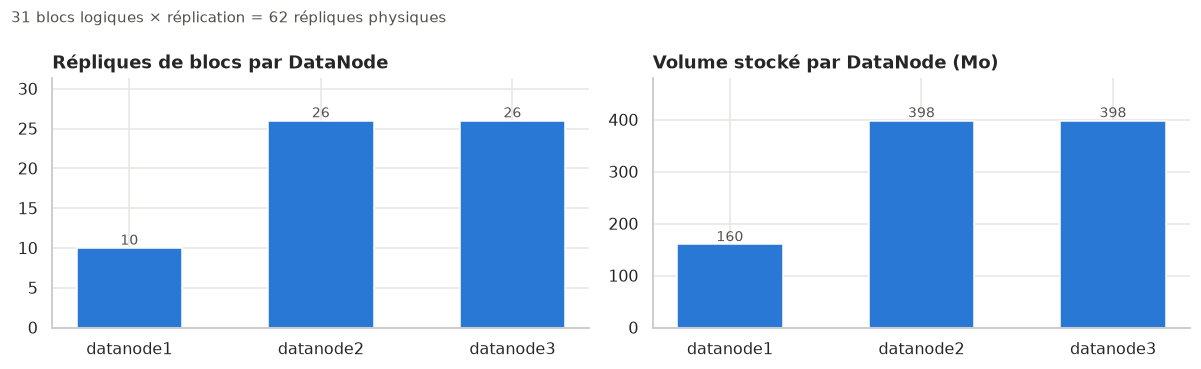
\includegraphics[width=\linewidth]{figures/j1_c08.png}
\caption{Répartition des 62 répliques sur les trois DataNodes.}
\end{figure}

Un fichier de 15 Ko n'occupe pas 16 Mo de disque : la taille de bloc est un maximum logique. En revanche, chaque fichier et chaque
bloc coûtent environ 150 octets de mémoire au NameNode, ce qui fonde le \emph{Small Files Problem} traité au Jour 3.

\subsection{Partitions Spark et localité des données}
Le nombre de partitions Spark n'est pas directement le nombre de blocs. Pour une source fichier, Spark découpe selon
\[ \text{split} = \min\Big(\texttt{maxPartitionBytes},\ \max\big(\texttt{openCostInBytes},\ \tfrac{\text{taille totale}}{\text{nb cœurs}}\big)\Big). \]
Par défaut (128 Mo, 8 cœurs), le fichier de 335 Mo est lu en \textbf{8 partitions}. En fixant \code{maxPartitionBytes = 16 Mo},
on obtient \textbf{21 partitions pour 21 blocs} : chaque tâche lit un bloc entier, idéalement sur le DataNode qui l'héberge.

\subsection{Crash-test réalisé sur le cluster}\label{sec:crash}
Le DataNode 2 a été arrêté brutalement (\code{docker stop datanode2}) pendant que le cluster contenait l'ensemble du Lakehouse.

\begin{table}[H]
\centering\small
\begin{tabularx}{\linewidth}{@{}l Y@{}}
\toprule
\textbf{Instant} & \textbf{Observation (mesures réelles)} \\ \midrule
T0 & 3 DataNodes vivants, 0 bloc sous-répliqué \\
T + 0 s & arrêt brutal de \code{datanode2} \\
T + 49 s & \code{datanode2} déclaré \textbf{mort} par le NameNode (théorie : 50 s) ; 314 blocs sous-répliqués \\
T + 75 s & lecture complète de \code{fraud\_train.csv} par Spark pendant la panne : \textbf{1\,296\,675 lignes}, aucune erreur \\
T + 260 s & \code{fsck} : statut \textbf{HEALTHY}, 0 bloc manquant, 0 bloc corrompu ; ré-réplication en cours \\
T + 267 s & redémarrage du nœud : 3 DataNodes vivants, \textbf{0 bloc sous-répliqué} \\
\bottomrule
\end{tabularx}
\caption{Chronologie du crash-test.}
\end{table}

\begin{keybox}[Analyse]
La seconde réplique de chaque bloc garantit la continuité de service. La ré-réplication vers le DataNode survivant est
volontairement bridée par HDFS (2 flux par nœud par défaut, \code{dfs.namenode.replication.max-streams}) pour ne pas saturer le
réseau : avec 314 blocs à recopier, elle prend plusieurs minutes. Au redémarrage, le \emph{block report} du nœud restauré suffit à
retrouver instantanément le facteur de réplication cible.
\end{keybox}

\subsection{Couche Bronze}
Les sources sont converties en tables Delta enrichies de colonnes de lignage (\code{\_ingested\_at}, \code{\_source\_dataset},
\code{\_source\_file}, \code{\_batch\_id}). Choix d'ingénierie : \textbf{schéma explicite} pour les transactions (pas de double
lecture pour \code{inferSchema}, numéro de carte et code postal conservés en chaîne), et ingestion des deux fichiers dans une seule
table, l'origine restant traçable. Résultat : \code{bronze/transactions} (1\,852\,394 lignes) et \code{bronze/us\_holidays}
(342 lignes) ; le format Parquet compressé réduit l'empreinte de 478 Mo à 144 Mo (÷\,3,3).

% =====================================================================================
\section{Jour 2 — Couche Silver : qualité, features et garanties ACID}\label{sec:j2}

\subsection{Évaluation paresseuse}
Déclarer des transformations ne prend que 80 ms (aucun job lancé) ; l'action \code{count()} déclenche le calcul (3,5 s).
L'opérateur \code{Exchange} (\emph{shuffle}) n'apparaît que dans le plan de la transformation \emph{wide} (\code{groupBy}).

\subsection{Diagnostic qualité}
\begin{table}[H]
\centering\small
\begin{tabularx}{\linewidth}{@{}l l Y@{}}
\toprule
\textbf{Constat} & \textbf{Mesure} & \textbf{Décision} \\ \midrule
Valeurs manquantes & 0 \code{NULL}, 0 vide masqué & règle de nettoyage conservée par sécurité \\
Doublons & 0 sur \code{trans\_num} & dédoublonnage maintenu (idempotence) \\
Déséquilibre & 0,521\,\% de fraudes & métriques adaptées (PR-AUC), sous-échantillonnage \\
\code{unix\_time} incohérent & décalé de \textbf{7 ans} & colonne écartée, epoch recalculé \\
Préfixe artificiel & 100\,\% des marchands en \code{fraud\_} & préfixe supprimé \\
Calendrier & dates en double (Pâques) & pré-agrégation par date avant jointure \\
\bottomrule
\end{tabularx}
\caption{Anomalies détectées et traitements appliqués.}
\end{table}

\subsection{Ingénierie des variables}
Vingt variables sont créées, dont cinq de \textbf{vélocité} calculées par fonctions de fenêtrage partitionnées par carte :
nombre et montant cumulé des transactions sur 24 h (\code{rangeBetween(-86400, 0)}), délai depuis la transaction précédente
(\code{LAG}), moyenne historique de la carte et ratio du montant à cette moyenne. Toutes les fenêtres ne regardent que le
\textbf{passé} de la carte : aucune fuite d'information vers le modèle. La distance domicile--commerçant est calculée par la formule
de Haversine.

\subsection{Jointure multi-sources sans explosion N-à-M}\label{sec:join}
Une même date peut se trouver dans la fenêtre de plusieurs jours fériés (24 décembre : veille de Noël, J-1 de Noël…).
Une dimension calendrier à \textbf{clé unique} est donc construite par pré-agrégation (\code{min\_by}), puis diffusée
(\code{BroadcastHashJoin}).

\begin{center}
\begin{tabular}{@{}l r@{}}
\toprule
Transactions avant jointure & 1\,852\,394 \\
Jointure naïve sur le calendrier non agrégé & 2\,055\,483 \ (\textcolor{fl-orange}{+203\,089 lignes fantômes}) \\
Jointure sur la dimension à clé unique & \textbf{1\,852\,394} \\
\bottomrule
\end{tabular}
\end{center}

\subsection{Valeurs extrêmes : IQR contre Z-score}
Le seuil IQR ($Q_3 + 1{,}5\,\text{IQR} = 193$ \$) signale 5,1\,\% des transactions, le Z-score (548 \$) seulement 1,0\,\% : l'écart-type
gonflé par la longue traîne masque toute la zone 193--548 \$. Or les transactions « outliers IQR seulement » présentent déjà
3,5\,\% de fraude (7 fois le taux de base) et celles signalées par les deux méthodes 25,9\,\%. Les indicateurs sont conservés comme
variables : en détection de fraude, les valeurs extrêmes \emph{sont} le signal.

\begin{figure}[H]
\centering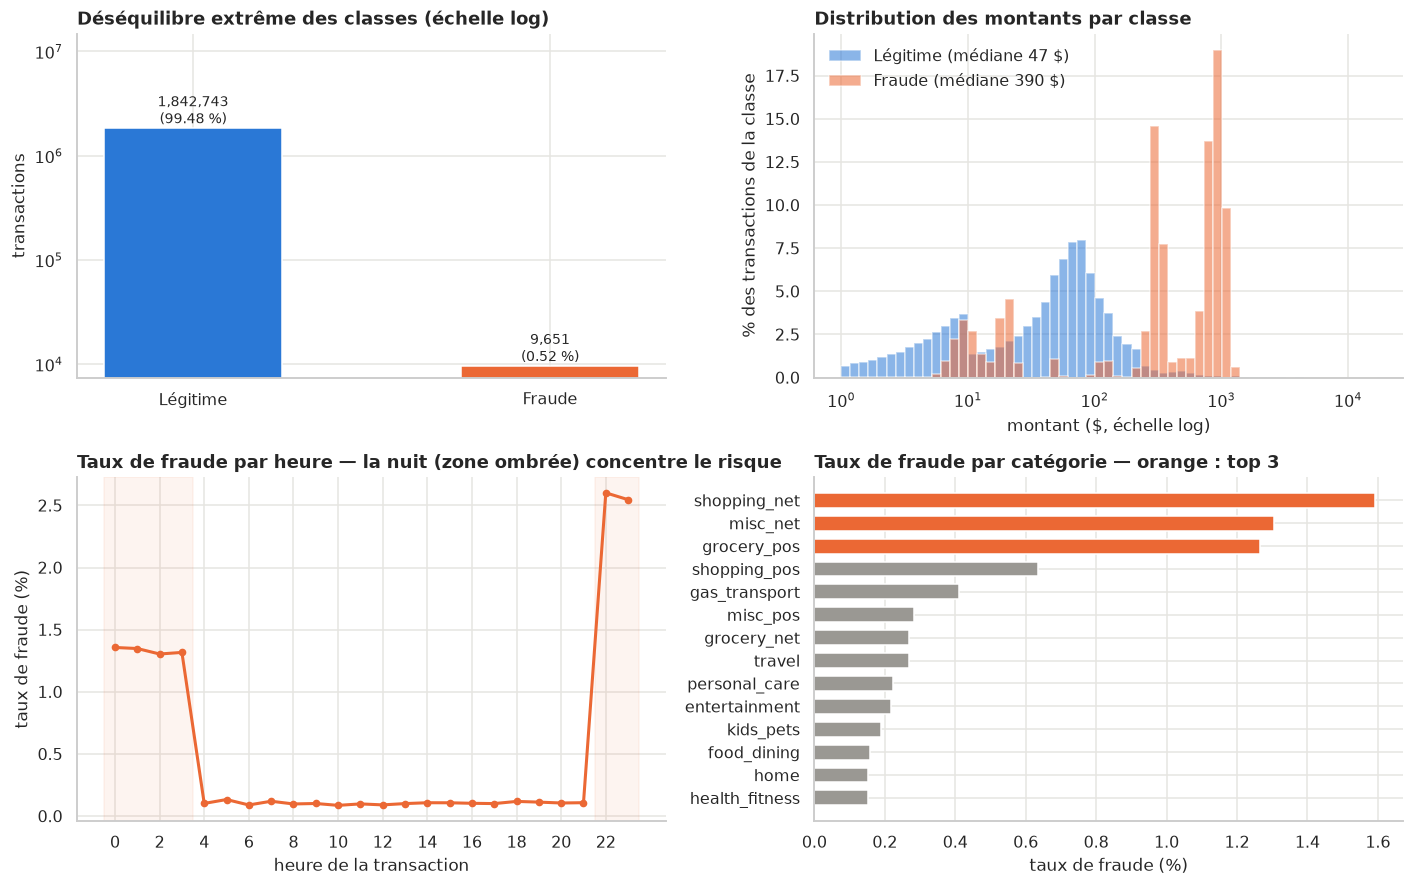
\includegraphics[width=0.94\linewidth]{figures/j2_c15.png}
\caption{Analyse exploratoire de la couche Silver.}
\end{figure}

\subsection{Garanties ACID de Delta Lake}\label{sec:acid}
\begin{itemize}[leftmargin=*,itemsep=2pt]
  \item \textbf{Journal transactionnel} : le commit 0 enregistre l'écriture de 216 fichiers Parquet partitionnés par mois.
  \item \textbf{Schema Enforcement} : un lot au schéma incompatible est rejeté atomiquement (\code{DELTA\_METADATA\_MISMATCH}).
  \item \textbf{MERGE INTO} : scénario métier d'un lot de 25 \emph{chargebacks} (fraudes confirmées tardivement) et d'une transaction
        arrivée en retard, avec élagage des partitions sur \code{trans\_month}.
  \item \textbf{Time Travel} : 9\,651 fraudes en version 0 contre 9\,676 après le MERGE (+25), vérifié par \code{versionAsOf}.
  \item \textbf{RESTORE} : le lot s'avérant erroné, la table est restaurée en une opération (9\,651 fraudes retrouvées).
\end{itemize}

% =====================================================================================
\section{Jour 3 — Spark SQL avancé et couche Gold}\label{sec:j3}

\subsection{Asymétrie et indicateurs robustes}
\begin{table}[H]
\centering\small
\begin{tabular}{@{}l r r r r r r r@{}}
\toprule
\textbf{Classe} & \textbf{n} & \textbf{Moyenne} & \textbf{Écart-type} & \textbf{Skewness} & \textbf{Médiane} & \textbf{IQR} & \textbf{P95} \\ \midrule
Légitime & 1\,842\,743 & 67,65 & 153,55 & 45,37 & 47,25 & 72,95 & 189,54 \\
Fraude & 9\,651 & 530,66 & 391,03 & 0,03 & 389,57 & 663,14 & 1\,084,02 \\
Ensemble & 1\,852\,394 & 70,06 & 159,25 & 40,81 & 47,45 & 73,44 & 195,23 \\
\bottomrule
\end{tabular}
\caption{Statistiques des montants (\$), une seule requête \code{GROUP BY GROUPING SETS}.}
\end{table}

Avec une asymétrie de 45, la moyenne décrit un client qui n'existe pas : la \textbf{médiane} et l'\textbf{IQR} sont retenus comme
indicateurs de référence. La fraude n'est pas seulement décalée (médiane 8 fois supérieure) : sa distribution est multimodale,
avec de petits montants de « test de carte » puis des paliers vers 300 \$ et 1\,000 \$, sous un plafond net de 1\,376 \$.

\begin{figure}[H]
\centering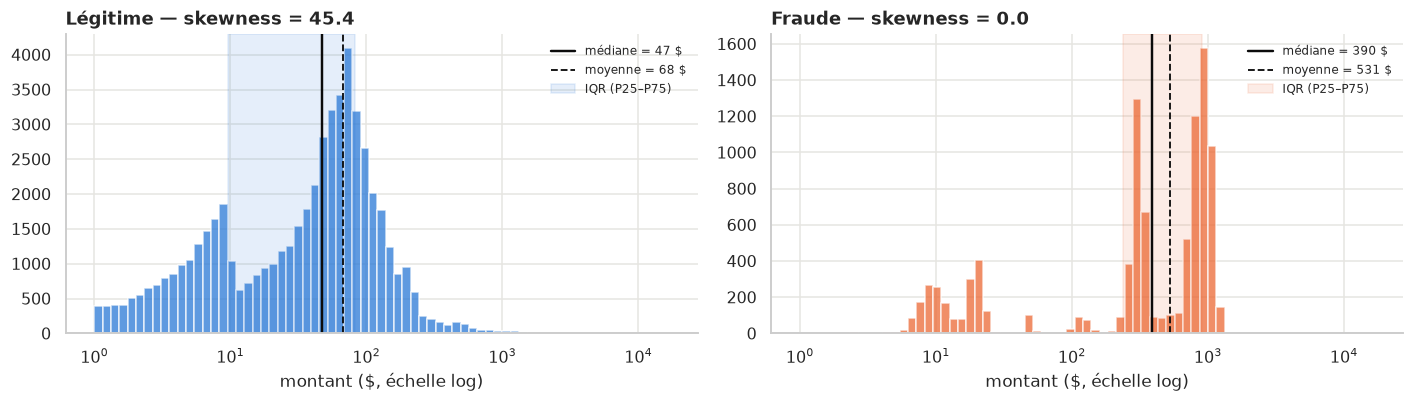
\includegraphics[width=0.95\linewidth]{figures/j3_c04.png}
\caption{Distribution des montants par classe : médiane, moyenne et IQR.}
\end{figure}

\subsection{Pareto des pertes}
Calculé par \code{SUM(fraud\_amount) OVER (ORDER BY fraud\_amount DESC ROWS BETWEEN UNBOUNDED PRECEDING AND CURRENT ROW)},
le cumul montre que \textbf{4 catégories sur 14} (\code{shopping\_net}, \code{misc\_net}, \code{shopping\_pos},
\code{grocery\_pos}) génèrent \textbf{93\,\%} des 5,12 M\$ fraudés.

\begin{figure}[H]
\centering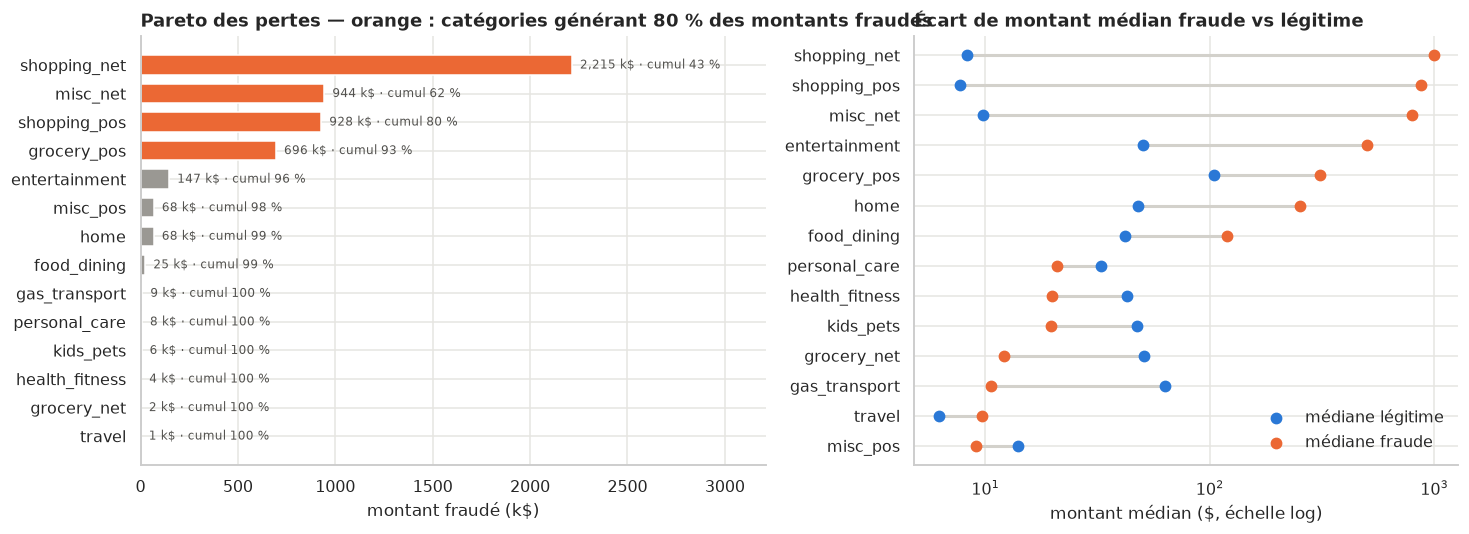
\includegraphics[width=\linewidth]{figures/j3_c07.png}
\caption{Pareto des pertes et écart de montant médian fraude / légitime par catégorie.}
\end{figure}

\subsection{Dynamique temporelle}
La moyenne glissante sur 7 jours lisse l'effet du jour de la semaine ; \code{LAG} mesure les variations hebdomadaires et mensuelles.
Le taux culmine en janvier--février 2019 (≈\,1\,\%). Décembre est un piège : le volume double et le \emph{nombre} de fraudes augmente
(+53\,\% en décembre 2019) alors que le \emph{taux} chute (0,42\,\% puis 0,19\,\%). La surveillance doit donc reposer sur le taux.

\begin{figure}[H]
\centering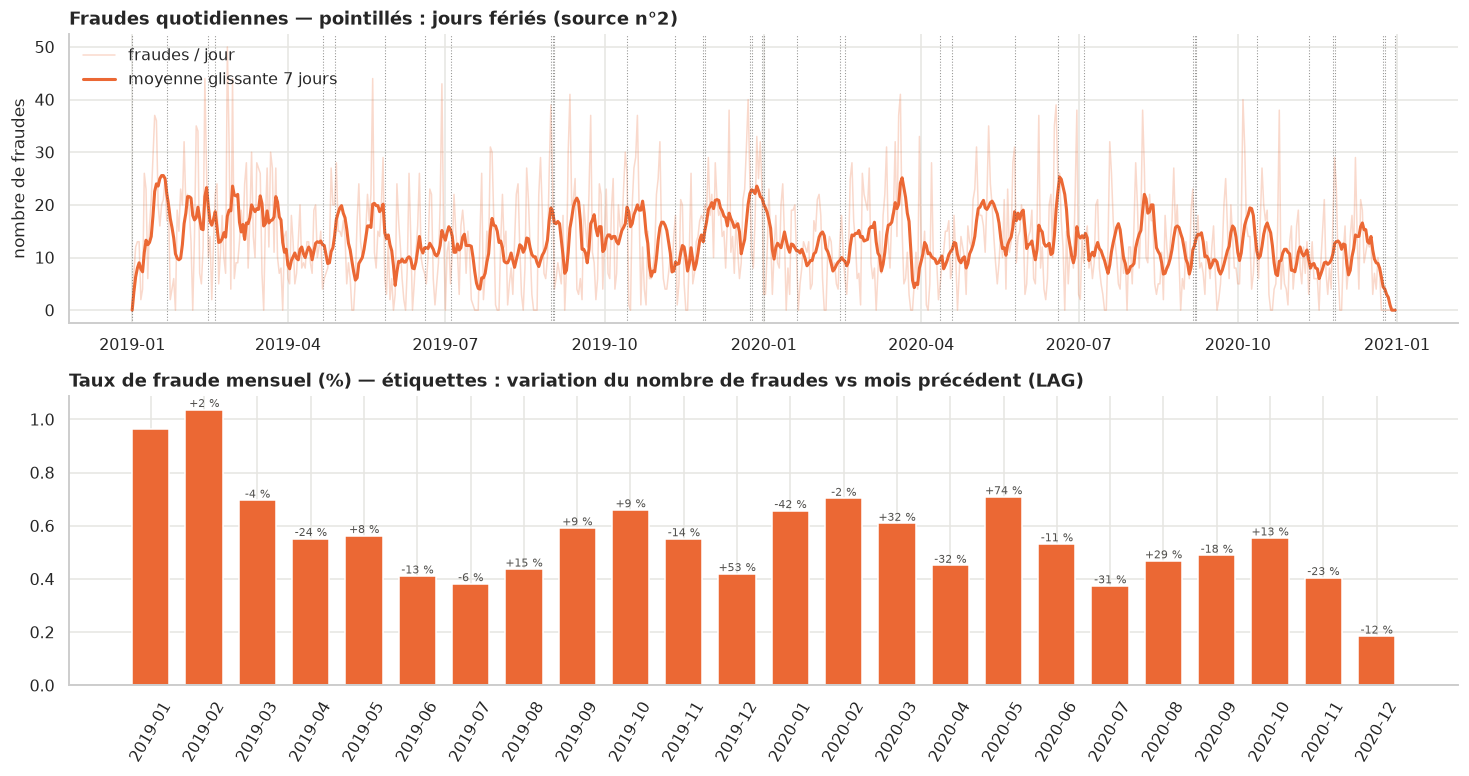
\includegraphics[width=\linewidth]{figures/j3_c10.png}
\caption{Fraudes quotidiennes (moyenne glissante 7 jours, jours fériés en pointillés) et taux mensuel.}
\end{figure}

\begin{figure}[H]
\centering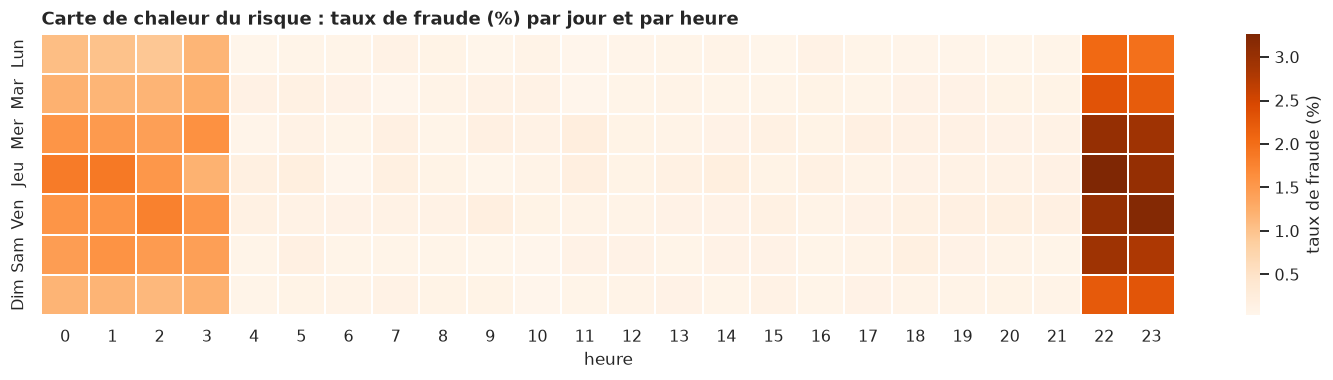
\includegraphics[width=\linewidth]{figures/j3_c13.png}
\caption{Carte de chaleur du risque : ≈\,2,5\,\% de fraude entre 22\,h et minuit contre ≈\,0,1\,\% en journée.}
\end{figure}

\subsection{Profil géographique et rigueur statistique}
Pour éviter de classer en tête un État à très faible volume, l'intervalle de confiance de Wilson~\cite{wilson1927} à 95\,\% est calculé directement en
SQL et le classement se fait sur sa borne basse ; la catégorie la plus fraudée de chaque État est obtenue par
\code{ROW\_NUMBER() OVER (PARTITION BY state ORDER BY n\_fraud DESC) = 1}.

\subsection{Compaction et catalogue}
\code{OPTIMIZE … ZORDER BY (card\_id)} réduit la table Silver de \textbf{216 à 24 fichiers} (163 Mo $\to$ 139 Mo) sans bloquer les
lecteurs. Chaque table Gold est documentée dans une table \code{data\_catalog} (description et requête SQL), que le tableau de bord
affiche sous chaque graphique.

% =====================================================================================
\section{Jour 4 — Tests d'hypothèses, segmentation et scoring}\label{sec:j4}

\subsection{Inférence statistique}\label{sec:tests}
Avec 1,85 M de lignes, presque tout devient significatif : chaque test est accompagné d'une \textbf{taille d'effet}. Les tableaux de
contingence des χ² sont calculés exactement par Spark ; les tests de rangs utilisent un échantillon stratifié (toutes les fraudes,
5\,\% des légitimes).

\begin{table}[H]
\centering\small
\begin{tabularx}{\linewidth}{@{}l Y r l l@{}}
\toprule
\textbf{Test} & \textbf{Question} & \textbf{p} & \textbf{Effet} & \textbf{Décision} \\ \midrule
Mann-Whitney U~\cite{mann1947} & montant fraude > légitime ? & $<10^{-300}$ & $r = 0{,}67$ (fort) & $H_0$ rejetée \\
χ² (2×2) & risque dépendant de la nuit ? & $<10^{-300}$ & RR = 18,0 ; V = 0,10 & $H_0$ rejetée \\
χ² (2×2) & jours fériés plus risqués ? (source 2) & 0,61 & RR = 0,99 ; V ≈ 0 & $H_0$ \textbf{non} rejetée \\
Kruskal-Wallis~\cite{kruskal1952} & montant des fraudes selon la catégorie ? & $<10^{-300}$ & $\varepsilon^2 = 0{,}90$ (fort) & $H_0$ rejetée \\
\bottomrule
\end{tabularx}
\caption{Résultats des tests d'hypothèses ($\alpha = 5\,\%$).}
\end{table}

\begin{warnbox}[Résultat négatif]
La proximité d'un jour férié ne modifie pas le risque (0,517\,\% contre 0,523\,\%) : volume légitime et fraude augmentent dans les
mêmes proportions. Ce résultat évite une règle anti-fraude « spéciale fêtes » qui n'aurait aucun fondement.
\end{warnbox}

\begin{figure}[H]
\centering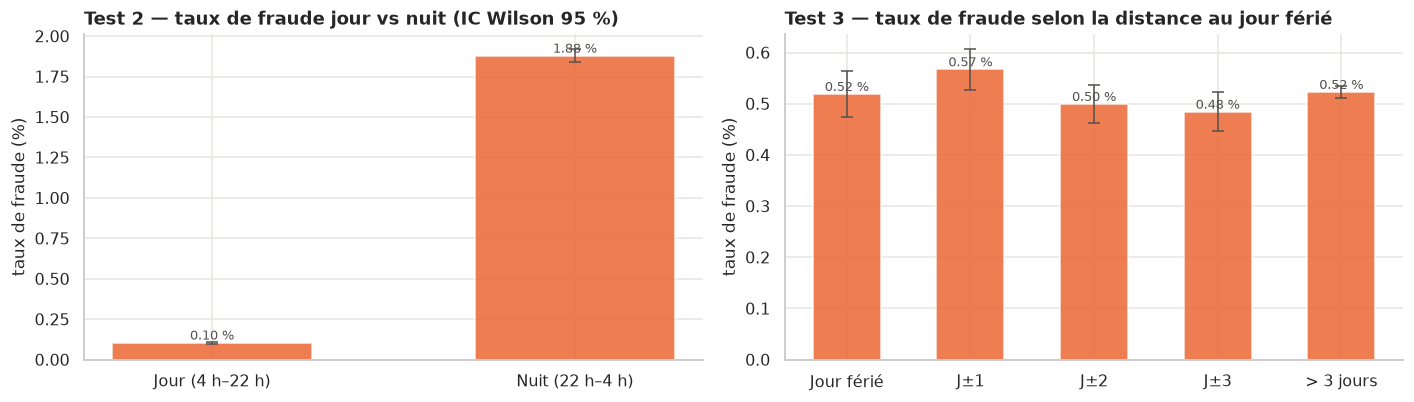
\includegraphics[width=0.95\linewidth]{figures/j4_c04.png}
\caption{Taux de fraude jour/nuit et selon la distance au jour férié (intervalles de Wilson).}
\end{figure}

\subsection{Segmentation des porteurs}
Les 999 cartes sont décrites par leur comportement \emph{légitime} (fréquence, panier médian, part e-commerce, part nocturne, âge),
puis segmentées par K-Means après \code{log1p} et standardisation. 91 cartes n'ont \textbf{aucune} transaction légitime (cartes
compromises dès l'émission) et sont traitées à part. Le nombre de segments ($k = 4$) suit une règle de parcimonie : la silhouette de
$k = 4$ (0,359) est à moins de 0,01 du maximum~\cite{rousseeuw1987}.

\begin{table}[H]
\centering\small
\begin{tabular}{@{}l r r r r r@{}}
\toprule
\textbf{Segment} & \textbf{Cartes} & \textbf{Tx / mois} & \textbf{Panier médian} & \textbf{Taux de fraude} & \textbf{Part des pertes} \\ \midrule
Gros paniers · Jeunes & 95 & 61 & 76 \$ & 0,59\,\% & 12\,\% \\
Seniors · Noctambules & 399 & 61 & 42 \$ & 0,58\,\% & 46\,\% \\
Petits paniers · Diurnes & 275 & 91 & 35 \$ & 0,42\,\% & 32\,\% \\
Connectés e-commerce · Diurnes & 139 & 91 & 54 \$ & 0,33\,\% & 11\,\% \\
\bottomrule
\end{tabular}
\caption{Profils des segments et exposition à la fraude.}
\end{table}

Presque toutes les cartes (≈\,97\,\%) subissent au moins une fraude, avec un nombre quasi constant de fraudes par carte : les
fraudeurs ne choisissent pas leurs victimes. Mais le \emph{taux} est 1,4 à 1,8 fois plus élevé chez les porteurs peu actifs, où la
même rafale pèse davantage — d'où l'intérêt de seuils relatifs à l'historique de chaque carte.

\subsection{Premier modèle de scoring}
Un modèle \emph{Gradient-Boosted Trees} (Spark MLlib), entraîné jusqu'en juin 2020 et évalué sur la période suivante, atteint une
PR-AUC de 0,893 (231 fois le hasard) ; cette métrique est préférée à l'aire sous la courbe ROC, trop optimiste lorsque la classe d'intérêt est rare~\cite{saito2015}. Au seuil optimal, il détecte 78\,\% des fraudes et 86\,\% du montant fraudé, avec 89\,\% d'alertes
justifiées. Ce modèle est industrialisé au Jour 5.

% =====================================================================================
\section{Jour 5 — Industrialisation MLOps}\label{sec:j5}

\begin{figure}[H]
\centering
\begin{tikzpicture}[font=\sffamily\small,node distance=4mm,
  st/.style={draw=fl-navy!45,fill=fl-light,rounded corners=3pt,minimum height=12mm,text width=22mm,align=center},
  arr/.style={-{Stealth[length=2mm]},thick,color=fl-navy!70}]
  \node[st] (d) {\textbf{Données}\\\footnotesize Silver v.\,figée};
  \node[st,right=of d] (e) {\textbf{① Expériences}\\\footnotesize 5 candidats};
  \node[st,right=of e,fill=fl-sand,draw=fl-orange] (q) {\textbf{② Portes}\\\footnotesize perf. + équité};
  \node[st,right=of q] (r) {\textbf{③ Registre}\\\footnotesize @champion};
  \node[st,right=of r] (p) {\textbf{④ Déploiement}\\\footnotesize HDFS + API};
  \node[st,below=7mm of p] (b) {\textbf{⑤ Scoring}\\\footnotesize file d'alertes};
  \node[st,left=of b] (m) {\textbf{⑥ Surveillance}\\\footnotesize PSI, perf.};
  \foreach \a/\b in {d/e,e/q,q/r,r/p,p/b,b/m} \draw[arr] (\a) -- (\b);
  \draw[arr,dashed,fl-orange] (m.west) -| node[pos=0.25,below,font=\sffamily\scriptsize,text=fl-orange]{dérive ≥ 0,25 : ré-entraînement} (e.south);
\end{tikzpicture}
\caption{Cycle de vie MLOps mis en œuvre.}
\end{figure}

\subsection{Principes}
Un modèle performant dans un notebook n'est pas un système de production : l'essentiel de la dette technique se situe autour du
modèle (données, configuration, surveillance)~\cite{sculley2015}. Les choix suivants y répondent.
\begin{itemize}[leftmargin=*,itemsep=2pt]
  \item \textbf{Reproductibilité} : la version Delta de la Silver est figée et journalisée (\code{versionAsOf}).
  \item \textbf{Validation sans fuite} : train (2019-01 → 2020-04), validation (2020-05 → 2020-06), test (2020-06 → 2020-12) ; le seuil
        et le modèle sont choisis sur la validation, la performance est mesurée une seule fois sur le test.
  \item \textbf{Pas d'écart entraînement / production} : features, motifs d'alerte et seuils sont définis une seule fois dans le
        package \code{fraudlake/}, partagé par le notebook, le scoring batch et l'API.
  \item \textbf{Qualité logicielle} : 33 tests unitaires (\code{pytest}) et intégration continue GitHub Actions (\code{ruff} + tests).
\end{itemize}

\subsection{Expériences suivies dans MLflow}
Chaque entraînement est journalisé dans MLflow~\cite{zaharia2018} (paramètres, métriques, version des données, artefacts).
\begin{table}[H]
\centering\small
\begin{tabular}{@{}l r r r r r r r@{}}
\toprule
\textbf{Candidat} & \textbf{PR-AUC val.} & \textbf{PR-AUC test} & \textbf{Seuil} & \textbf{Précision} & \textbf{Rappel} & \textbf{Équité 4/5} & \textbf{Portes} \\ \midrule
Régression logistique & 0,542 & 0,403 & 0,56 & 45\,\% & 66\,\% & 0,84 & \ko \\
Forêt aléatoire & 0,937 & 0,898 & 0,68 & 83\,\% & 86\,\% & 0,88 & \ok \\
GBT v1 (modèle J4) & 0,933 & 0,889 & 0,80 & 80\,\% & 85\,\% & 0,88 & \ok \\
\rowcolor{fl-sand}\textbf{GBT v2} & \textbf{0,956} & \textbf{0,926} & 0,88 & \textbf{89\,\%} & 86\,\% & 0,87 & \ok \\
GBT v2 sans genre & 0,954 & 0,923 & 0,88 & 88\,\% & 85\,\% & 0,85 & \ok \\
\bottomrule
\end{tabular}
\caption{Comparaison des cinq candidats (sélection sur la PR-AUC de validation).}
\end{table}

\begin{figure}[H]
\centering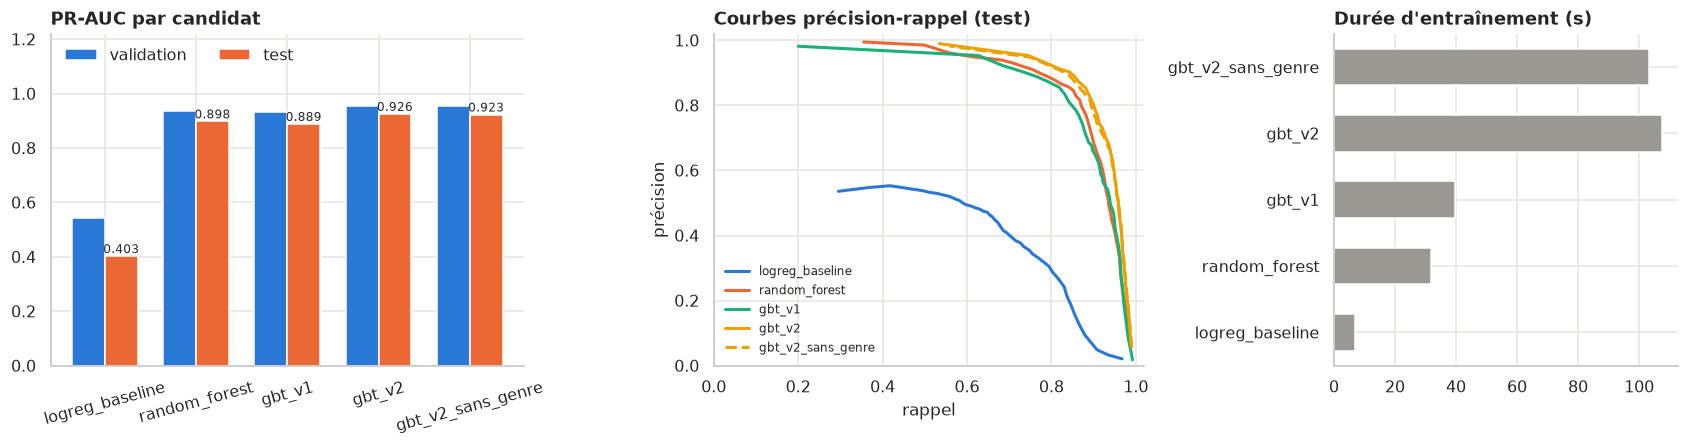
\includegraphics[width=\linewidth]{figures/j5_c09.png}
\caption{PR-AUC, courbes précision-rappel et durées d'entraînement des candidats.}
\end{figure}

Les modèles d'arbres dépassent largement la référence linéaire : la fraude dépend d'interactions non linéaires (montant × nuit ×
catégorie × vélocité). Ils restent très proches entre eux, ce qui justifie de toujours choisir sur la validation.

\subsection{Portes de qualité et équité}
Un candidat n'est promouvable que s'il atteint une PR-AUC $\geq 0{,}75$, un rappel $\geq 70\,\%$, une précision $\geq 50\,\%$ et
respecte la \textbf{règle des quatre cinquièmes}~\cite{eeoc1978} : le rappel du groupe le moins bien servi (genre, tranche d'âge) doit atteindre au
moins 80\,\% de celui du groupe le mieux servi.

\begin{figure}[H]
\centering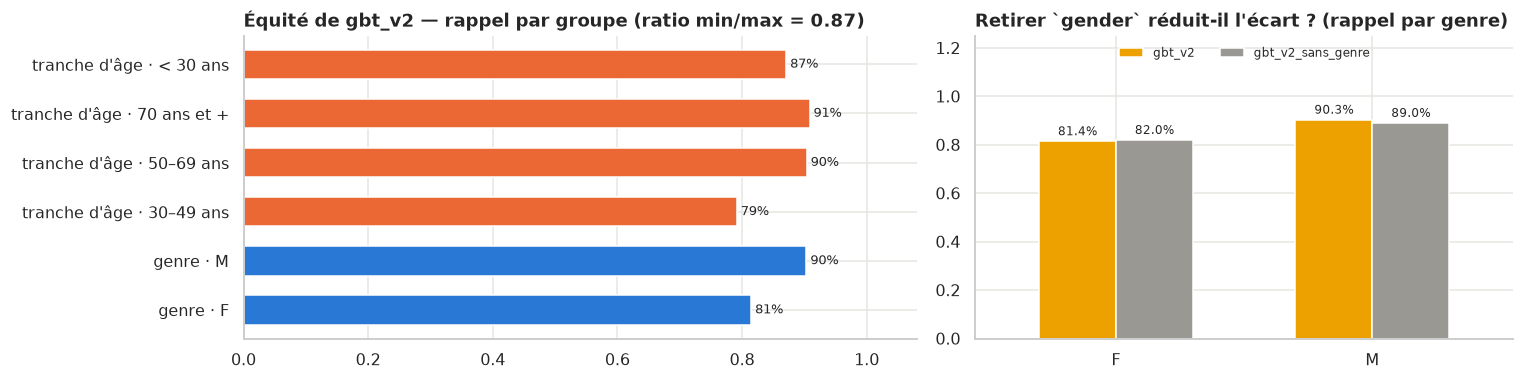
\includegraphics[width=\linewidth]{figures/j5_c12.png}
\caption{Rappel du champion par groupe et effet du retrait de la variable genre.}
\end{figure}

\begin{warnbox}[Équité]
Le champion détecte 81\,\% des fraudes visant des femmes contre 90\,\% pour les hommes, et 79\,\% pour les 30--49 ans contre 91\,\% pour
les 70 ans et plus (ratio 0,87, porte validée). Retirer la variable \code{gender} \emph{ne réduit pas} l'écart (ratio 0,85) : il provient
de profils de fraude différents selon les groupes. Supprimer une variable sensible ne suffit pas ; il faut mesurer le résultat à chaque
version, ce que font les portes.
\end{warnbox}

\subsection{Registre, déploiement et API}
Le candidat validé est enregistré dans le registre MLflow (\code{fraudlake-scoring}) et reçoit l'alias \code{@champion} ; le précédent
champion garde l'alias \code{@previous\_champion}, ce qui permet un retour arrière en une ligne. Le modèle est exporté sur HDFS avec ses
métadonnées et servi par l'API FastAPI, rechargée à chaud par \code{POST /reload}. Une fiche modèle (\emph{model card}~\cite{mitchell2019}) est générée
automatiquement.

\needspace{12\baselineskip}
\begin{lstlisting}[language=bash,caption={Appel réel de l'API de scoring.}]
POST http://localhost:8010/predict
{"category": "shopping_net", "amt": 962.4, "hour": 23, "amt_sum_24h": 2210.0,
 "amt_ratio_to_card_mean": 11.8, ...}

{"fraud_score": 0.98519, "decision": "ALERTE", "priority": "critique", "threshold": 0.88,
 "reasons": ["Montant élevé (962 $)", "Dépenses cumulées sur 24 h anormales (2210 $)",
             "Montant 11.8 fois supérieur à l'habitude de la carte",
             "Transaction nocturne (22 h – 4 h)", "Catégorie à risque élevé (shopping_net)"],
 "model_version": "1"}
\end{lstlisting}

\subsection{File d'alertes expliquées}
Le champion score six mois de transactions ; chaque alerte reçoit une priorité et des motifs lisibles issus de règles calibrées sur les
données (lift = taux de fraude ciblé / taux de base) : montant $\geq 500$ \$ (×41), cumul 24 h $\geq 1\,500$ \$ (×35), montant 4 fois
supérieur à l'habitude (×23), nuit (×3,6).

\begin{center}
\small
\begin{tabular}{@{}l r r r@{}}
\toprule
\textbf{Priorité} & \textbf{Alertes} & \textbf{Fraudes confirmées} & \textbf{Montant en jeu} \\ \midrule
Critique & 1\,507 & \textbf{97,1\,\%} & 915\,k\$ \\
Élevée & 557 & 66,4\,\% & 361\,k\$ \\
\bottomrule
\end{tabular}
\end{center}
99,7\,\% des alertes portent au moins un motif explicatif.

\subsection{Surveillance en production}
La dérive de chaque variable est mesurée chaque mois par le \emph{Population Stability Index}~\cite{siddiqi2006}, sur les déciles de la période
d'entraînement :
\[ \text{PSI} = \sum_i (p_i^{\text{prod}} - p_i^{\text{réf}}) \ln\frac{p_i^{\text{prod}}}{p_i^{\text{réf}}}, \qquad
   \text{stable si} < 0{,}10,\ \text{dérive si} \geq 0{,}25. \]

\begin{figure}[H]
\centering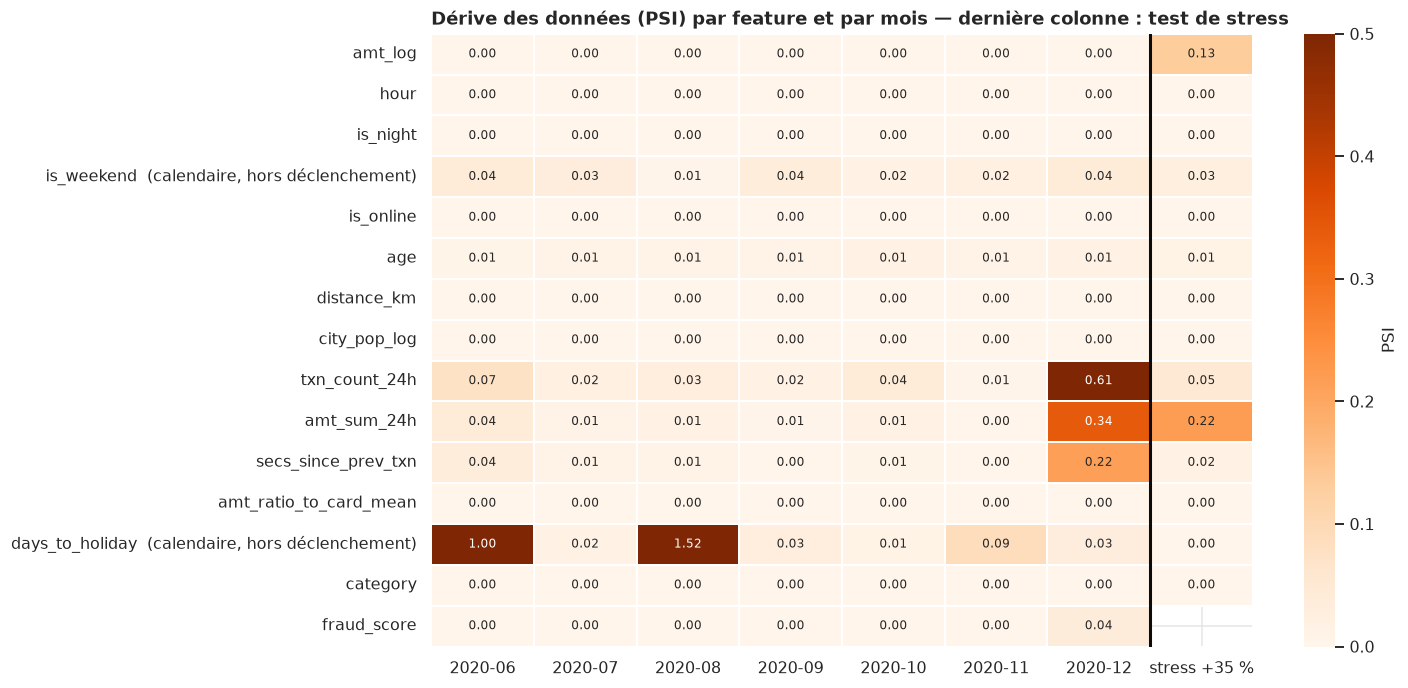
\includegraphics[width=\linewidth]{figures/j5_c23.png}
\caption{PSI par variable et par mois ; dernière colonne : test de stress (+35\,\% sur les montants).}
\end{figure}

\begin{table}[H]
\centering\small
\begin{tabular}{@{}l r r r r l@{}}
\toprule
\textbf{Période} & \textbf{Précision} & \textbf{Rappel} & \textbf{PR-AUC} & \textbf{PSI max} & \textbf{Décision} \\ \midrule
2020-06 à 2020-11 & 86--92\,\% & 84--88\,\% & 0,91--0,94 & $\leq 0{,}07$ & stable \\
2020-12 & 82,5\,\% & 84,1\,\% & 0,881 & 0,61 & \textbf{ré-entraînement} (dérive) \\
Stress +35\,\% & 39,5\,\% & 86,2\,\% & 0,680 & 0,22 & \textbf{ré-entraînement} (performance) \\
\bottomrule
\end{tabular}
\caption{Performance mensuelle et décisions de ré-entraînement.}
\end{table}

\begin{keybox}[Lecture]
(1) Les variables calendaires déterministes (\code{days\_to\_holiday}) varient mécaniquement (août ne contient aucun jour férié) : elles
sont affichées mais exclues du déclenchement, ce qui évite des fausses alertes. (2) Décembre présente une vraie dérive saisonnière des
variables de vélocité (achats de Noël) qui dégrade la précision : le ré-entraînement est légitime. (3) Le test de stress montre la
complémentarité des signaux : la dérive des données reste modérée mais la précision s'effondre, et c'est la règle de performance qui
déclenche.
\end{keybox}

\begin{figure}[H]
\centering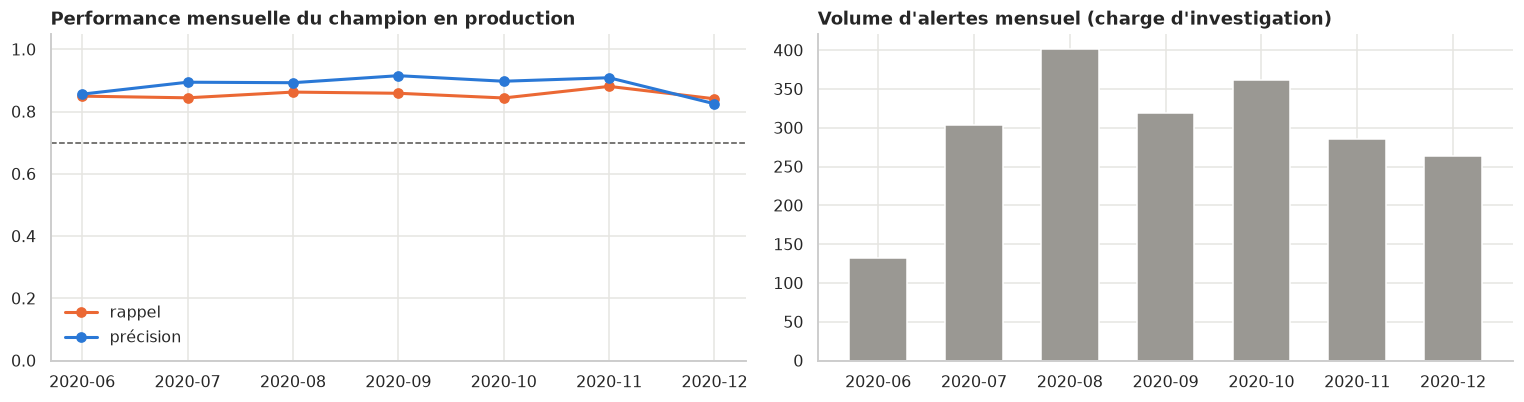
\includegraphics[width=\linewidth]{figures/j5_c24.png}
\caption{Performance mensuelle du champion et volume d'alertes.}
\end{figure}

% =====================================================================================
\section{Tableau de bord}\label{sec:dash}
Le tableau de bord Streamlit (\url{http://localhost:8501}) est la couche de restitution destinée aux équipes métier. Il ne lit que la
couche Gold : aucune donnée personnelle ni calcul lourd n'est exposé. Une barre latérale donne accès à douze pages et aux filtres
communs (période, catégories, coût d'investigation d'une alerte). Chaque graphique est accompagné d'un encadré présentant la requête
SQL source (issue de \code{data\_catalog}) et sa justification statistique.

\begin{table}[H]
\centering\small
\begin{tabularx}{\linewidth}{@{}l Y l@{}}
\toprule
\textbf{Page} & \textbf{Contenu} & \textbf{Question métier} \\ \midrule
Vue d'ensemble & chiffres clés filtrables, série quotidienne, taux mensuel, quartiles des montants & quelle est l'ampleur ? \\
Recherche de transactions & recherche plein texte, filtres (statut, canal, montant, période), fiche détaillée avec décision du modèle & que s'est-il passé sur cette transaction ? \\
Catégories & Pareto des pertes, médianes fraude / légitime, distributions & où perd-on de l'argent ? \\
Temporalité & carte de chaleur jour × heure, profil horaire & quand renforcer les contrôles ? \\
Géographie & carte des États, classement avec intervalles de confiance & où le risque est-il avéré ? \\
Segments clients & projection ACP, exposition par segment & quels clients protéger ? \\
Modèle de scoring & simulateur de seuil et gain net & quel seuil choisir ? \\
Scoring temps réel & appel de l'API du champion : jauge, verdict, motifs & que décide le modèle ? \\
Tests statistiques & quatre tests avec tailles d'effet & les écarts sont-ils réels ? \\
File d'alertes & flux de détection (Sankey), alertes priorisées, export CSV & que traiter en premier ? \\
MLOps & cycle de vie, expériences, registre, dérive, équité & le modèle reste-t-il fiable ? \\
Données & couches Médaillon, catalogue des tables Gold & d'où viennent les chiffres ? \\
\bottomrule
\end{tabularx}
\caption{Les douze pages du tableau de bord et la question à laquelle chacune répond.}
\end{table}

\begin{figure}[htbp]
\centering\fbox{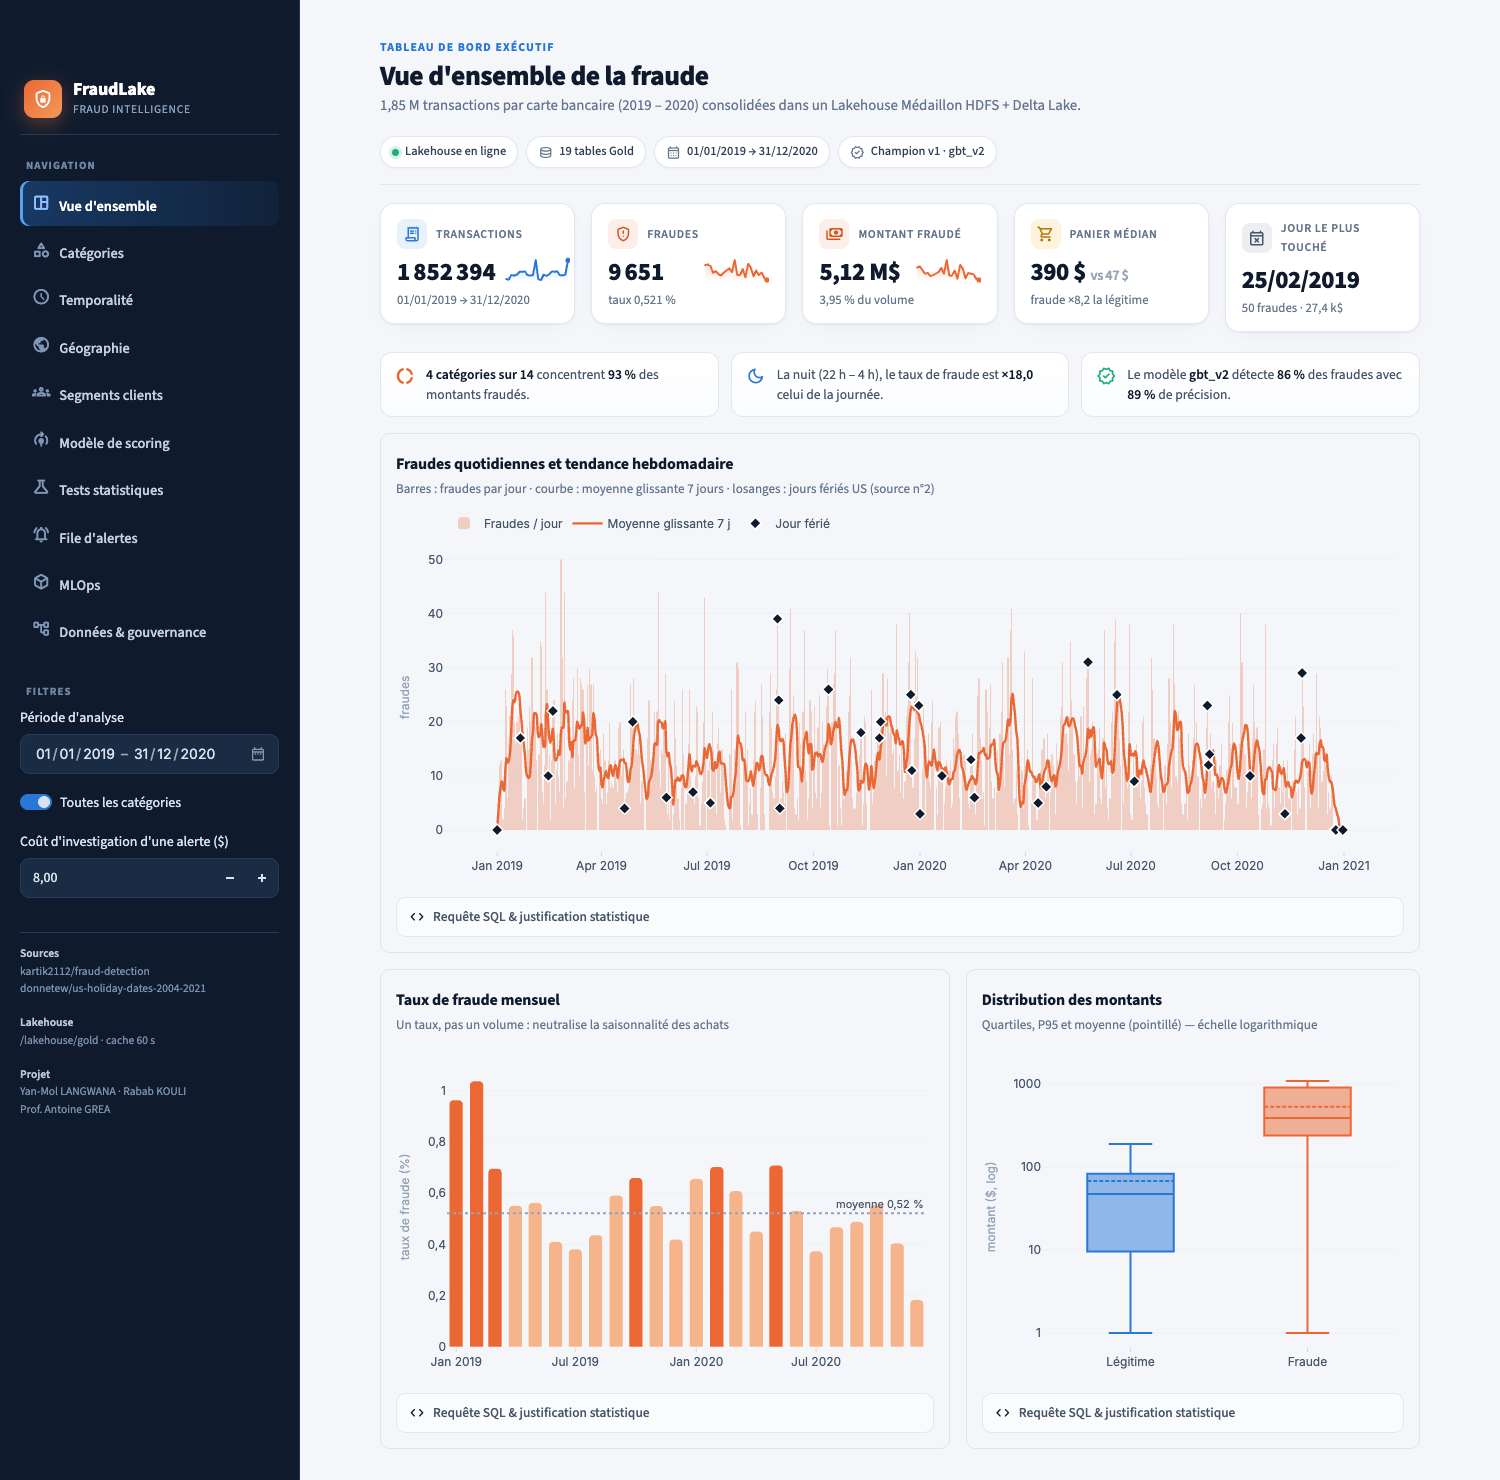
\includegraphics[width=0.97\linewidth]{figures/dash_overview.png}}
\caption{Page « Vue d'ensemble » : chiffres clés avec évolution mensuelle, points clés calculés sur les données, série quotidienne
avec jours fériés, taux mensuel et distribution des montants.}
\end{figure}

\textbf{Principes de conception.} Une couleur garde le même sens partout (bleu = légitime, orange = fraude) ; on affiche des
\emph{taux} plutôt que des volumes bruts ; chaque page commence par trois constats chiffrés générés à partir des tables Gold, pour que
le lecteur sache immédiatement quoi retenir ; les nombres suivent la typographie française (0,52\,\%, 1\,852\,394).

\textbf{Console d'investigation.} La page « Recherche de transactions » reprend les codes d'un backoffice de paiement : recherche
plein texte (référence, commerçant, catégorie, État), filtres par statut, canal, montant et période, tableau trié par date, et fiche
détaillée ouverte au clic. La fiche affiche la décision du modèle champion (score, priorité, motifs) ou, à défaut, les signaux de
risque évalués avec les mêmes seuils que l'API. Les volumes et taux sont pondérés par le plan de sondage de l'échantillon Gold, si
bien que le taux de fraude affiché (0,52\,\%) est celui de la population complète.

\begin{figure}[htbp]
\centering\fbox{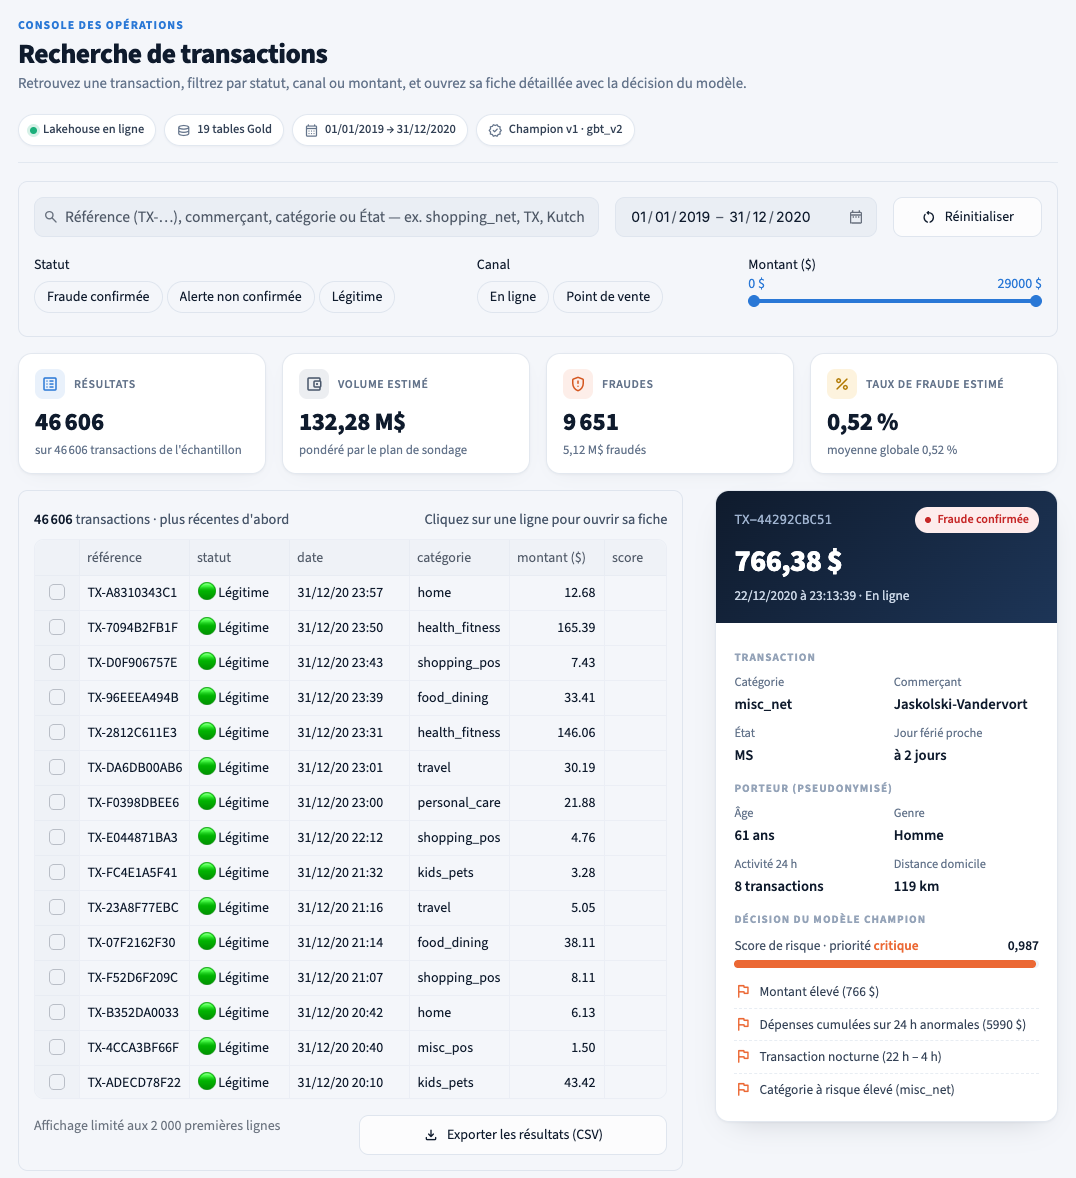
\includegraphics[width=0.92\linewidth]{figures/dash_search.png}}
\caption{Page « Recherche de transactions » : filtres, indicateurs recalculés sur la sélection, tableau des transactions et fiche
détaillée d'une fraude confirmée (score 0,987, priorité critique, quatre motifs).}
\end{figure}

\textbf{Démonstration de bout en bout.} La page « Scoring temps réel » envoie une transaction à l'API FastAPI qui sert le modèle
champion et affiche le score sur une jauge, la décision (bloquée ou acceptée), la priorité et les motifs d'alerte, avec la latence
mesurée. Trois scénarios prédéfinis (achat courant, achat nocturne en ligne, rafale de transactions) permettent de montrer en
direct le passage d'une transaction acceptée (score 0,014) à une transaction bloquée (score 0,985, cinq motifs).

\begin{figure}[htbp]
\centering\fbox{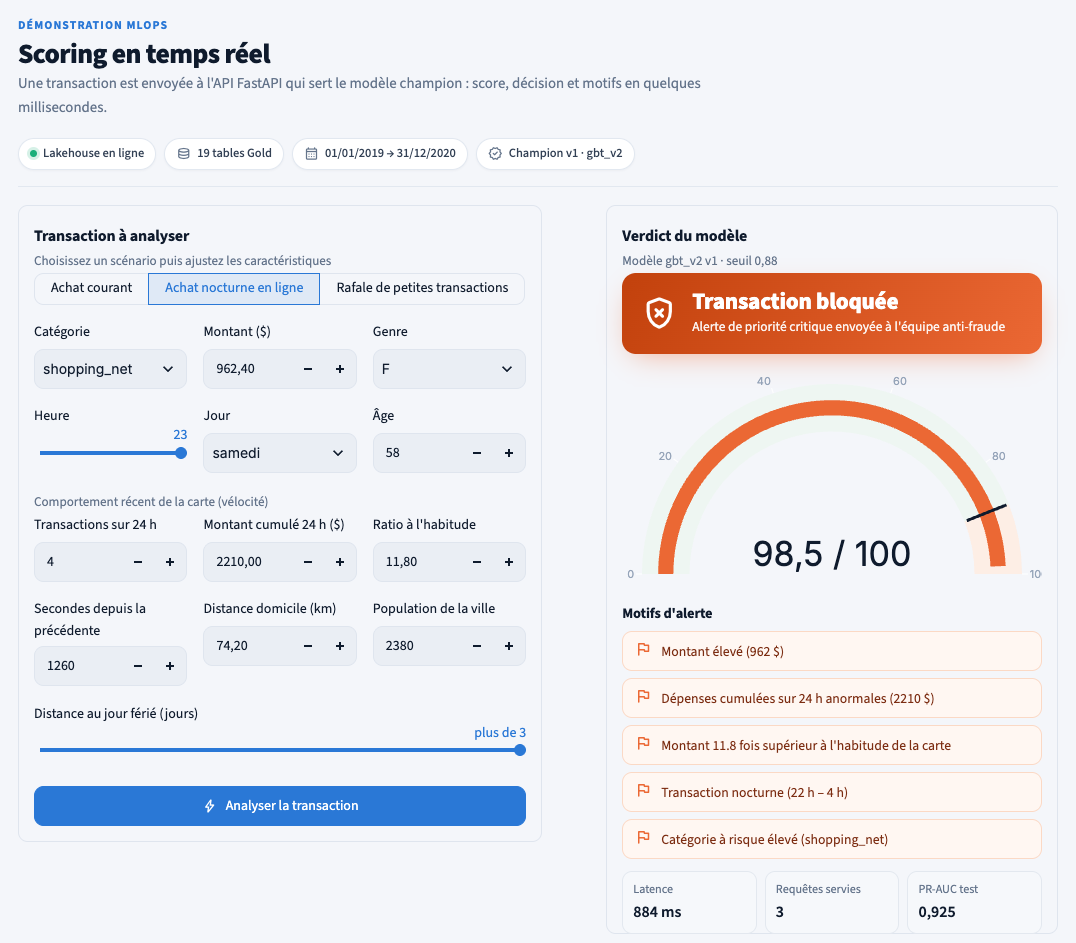
\includegraphics[width=0.9\linewidth]{figures/dash_live.png}}
\caption{Page « Scoring temps réel » : la transaction du scénario « achat nocturne en ligne » est envoyée à l'API ; le champion la
bloque (score 98,5/100, priorité critique) et justifie sa décision par cinq motifs lisibles.}
\end{figure}

\begin{figure}[htbp]
\centering
\fbox{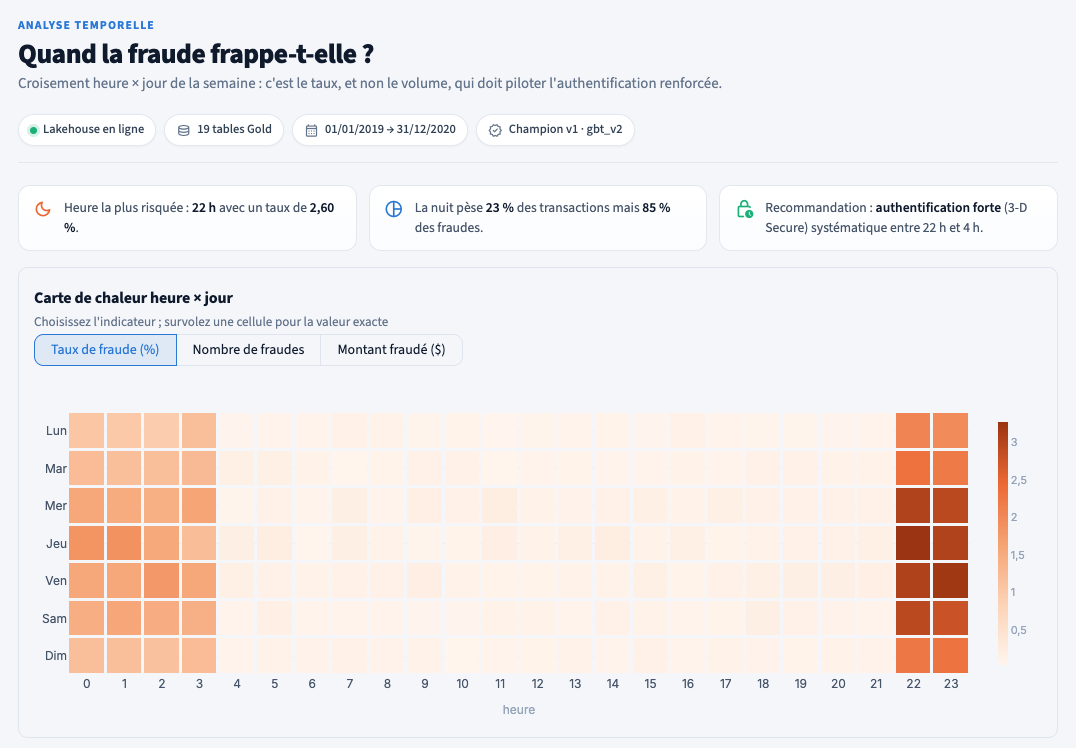
\includegraphics[width=0.48\linewidth]{figures/dash_time.png}}\hfill
\fbox{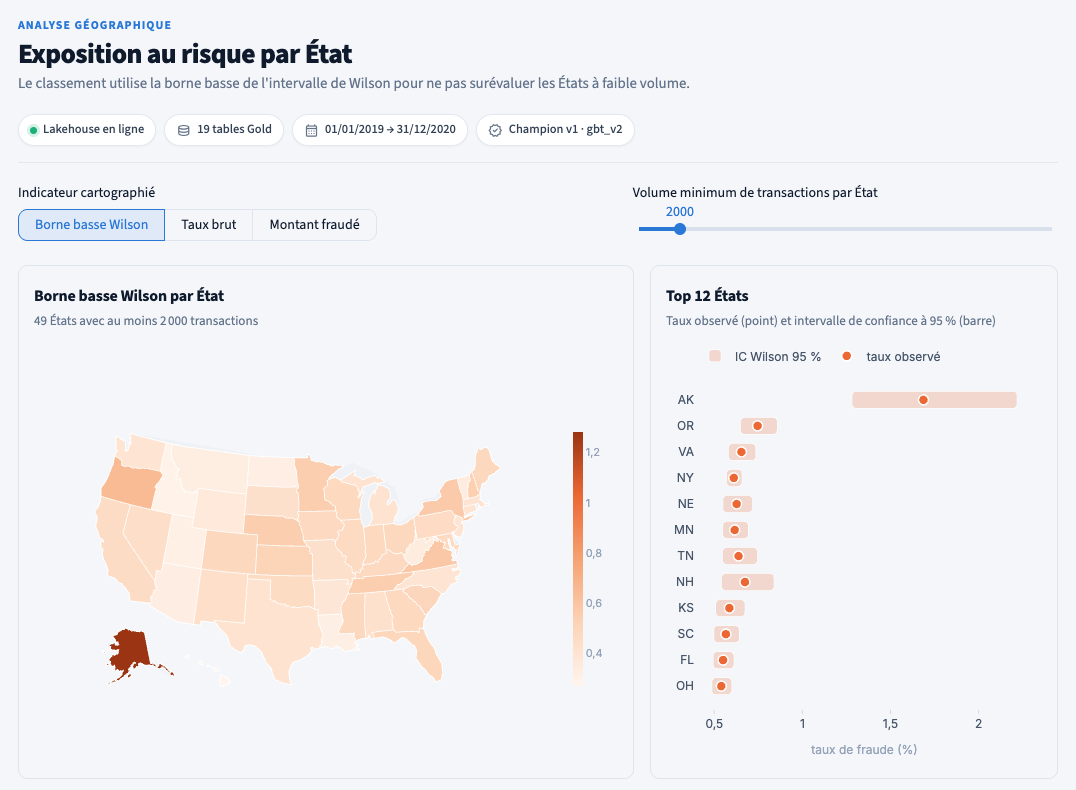
\includegraphics[width=0.48\linewidth]{figures/dash_geo.png}}
\caption{Pages « Temporalité » (carte de chaleur heure × jour) et « Géographie » (carte des États classés par borne basse de
Wilson).}
\vspace{10pt}
\centering\fbox{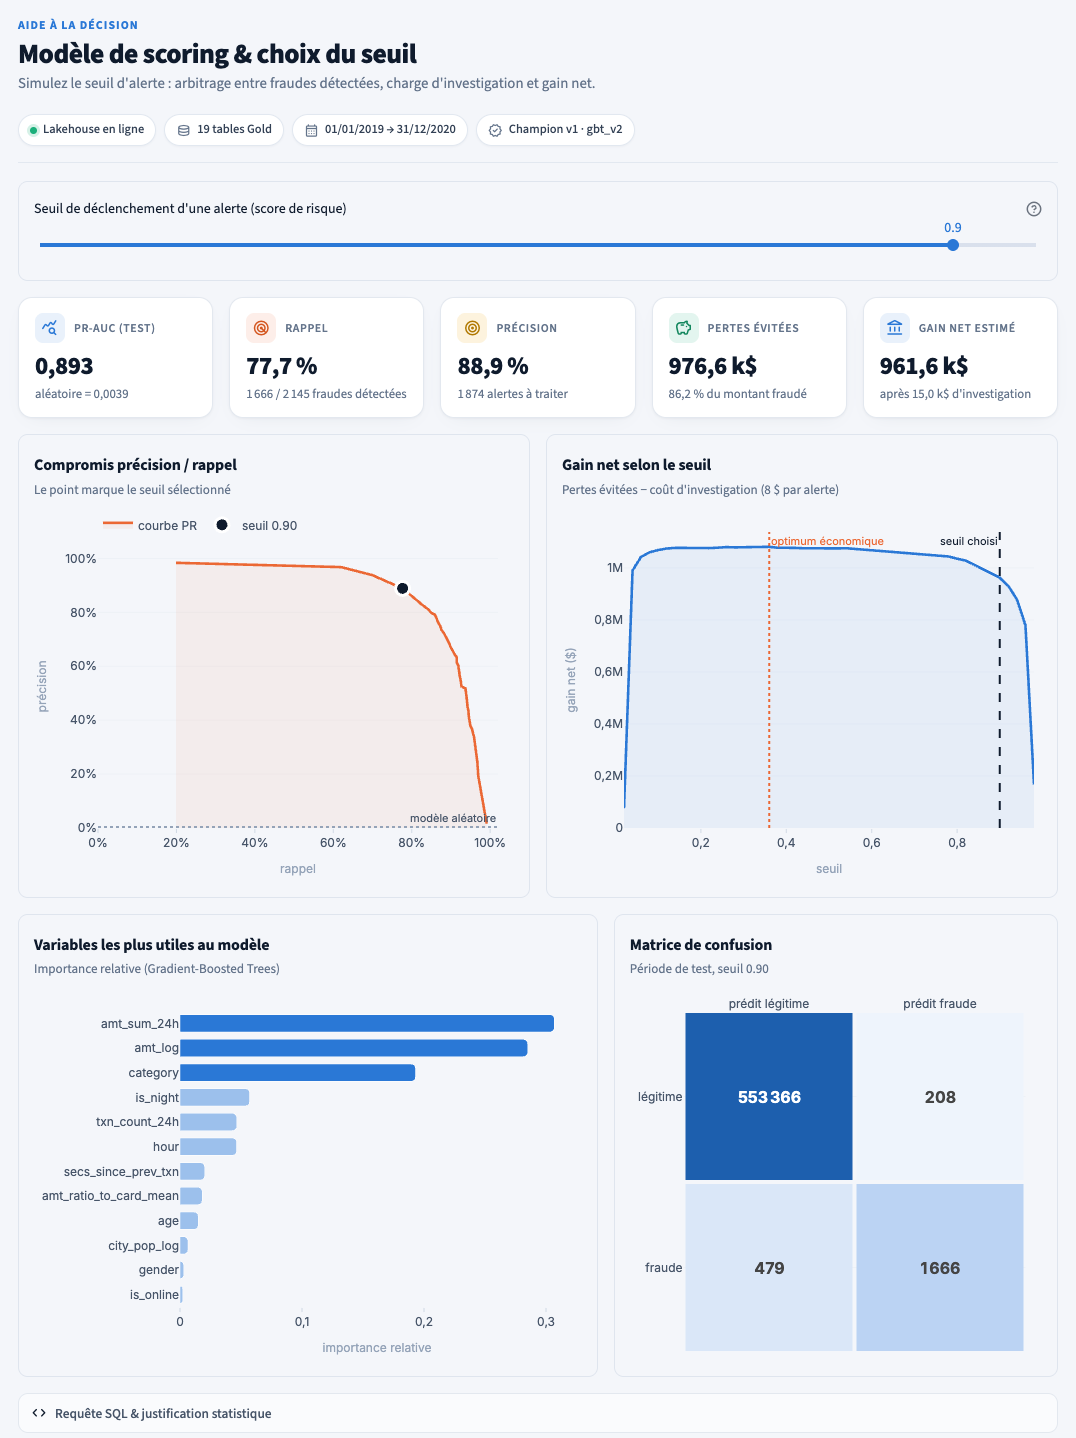
\includegraphics[width=0.64\linewidth]{figures/dash_model.png}}
\caption{Page « Modèle de scoring » : le curseur de seuil met à jour en direct le rappel, la précision, les pertes évitées et le gain
net, ainsi que la matrice de confusion.}
\end{figure}


% =====================================================================================
\clearpage
\section{Difficultés rencontrées et solutions}
\begin{table}[H]
\centering\small
\begin{tabularx}{\linewidth}{@{}l Y Y@{}}
\toprule
\textbf{Difficulté} & \textbf{Cause} & \textbf{Solution} \\ \midrule
Schéma erroné du calendrier & \code{DataFrameReader} mutable : le schéma des transactions était réutilisé & nouveau lecteur à chaque lecture \\
Horodatages incohérents & \code{unix\_time} décalé de 7 ans & colonne écartée, epoch recalculé \\
Doublons après jointure & fenêtres de jours fériés qui se chevauchent & dimension calendrier à clé unique \\
Arrêt brutal de Spark (OOM) & serveur MLflow à 2,3 Go (workers de tâches inutiles) & \code{MLFLOW\_SERVER\_ENABLE\_JOB\_EXECUTION=false} : 530 Mo \\
Échec d'écriture HDFS & disque virtuel Docker plein à 98\,\% & nettoyage du cache de construction (11 Go) \\
Ports déjà utilisés & 5000 réservé par AirPlay (macOS), 8000 par un autre projet & ports hôte 5050 et 8010, configurables \\
Porte d'équité refusée & écart de rappel de 10,6 points selon le genre & analyse (le retrait du genre ne corrige pas) et critère normatif des 4/5 \\
Fausses alertes de dérive & variables calendaires déterministes & exclusion du déclenchement \\
Services muets après un manque de mémoire & JVM Spark de l'API et du tableau de bord tuées ; état « ok » trompeur & contrôle de la JVM, auto-réparation, échecs exclus du cache \\
Rechargement du code ignoré & observateur de fichiers inopérant sur le volume Docker (macOS) & observation par scrutation (\code{fileWatcherType=poll}) \\
\bottomrule
\end{tabularx}
\caption{Principaux obstacles techniques.}
\end{table}

\textbf{Robustesse des services.} Lors des essais, la JVM Spark de l'API puis celle du tableau de bord ont été arrêtées par le
système faute de mémoire, alors que les deux services semblaient fonctionner : \code{/health} répondait « ok » et le tableau de bord
affichait à tort « tables Gold indisponibles ». Les deux services vérifient désormais que leur JVM répond et se réparent seuls :
nouvelle session Spark, rechargement du champion ou des tables, puis nouvelle tentative. Le tableau de bord distingue aussi une table
absente d'une panne du moteur, et n'enregistre plus un échec dans son cache. Vérification en tuant volontairement la JVM : réponse
correcte de l'API en 19\,s, page du tableau de bord rétablie en 70\,s.

% =====================================================================================
\section{Conclusion et recommandations}

\begin{table}[H]
\centering\small
\begin{tabularx}{\linewidth}{@{}c Y Y@{}}
\toprule
\textbf{\#} & \textbf{Constat établi} & \textbf{Recommandation} \\ \midrule
1 & risque ×18 entre 22\,h et 4\,h & authentification forte au-delà d'un montant la nuit \\
2 & montant médian frauduleux ×8, très variable selon la catégorie & seuils de montant par catégorie \\
3 & 4 catégories = 93\,\% des pertes & renforcer 3-D Secure sur \code{shopping\_net} et \code{misc\_net} \\
4 & aucun effet des jours fériés & pas de règle spécifique ; piloter sur le taux, pas le volume \\
5 & porteurs peu actifs plus exposés ; 91 cartes 100\,\% frauduleuses & seuils relatifs à l'historique ; contrôle à l'émission \\
6 & champion : PR-AUC 0,926, 97\,\% d'alertes critiques justes & déploiement en scoring temps réel, seuil fixé selon la capacité d'investigation \\
\bottomrule
\end{tabularx}
\caption{Synthèse des enseignements métier.}
\end{table}

Le projet démontre qu'une architecture \emph{Lakehouse} sur HDFS et Delta Lake réunit la robustesse d'un stockage distribué tolérant
aux pannes, les garanties transactionnelles d'une base de données (ACID, Time Travel) et la souplesse analytique de Spark. Le volet
MLOps transforme un modèle performant en un service gouverné : traçable, validé, équitable, explicable et surveillé.

\subsection*{Limites}
\begin{itemize}[leftmargin=*,itemsep=2pt]
  \item \textbf{Données synthétiques} : générées par le simulateur Sparkov, elles présentent des motifs plus nets qu'en réalité ; la
        PR-AUC de 0,926 serait sans doute plus basse sur des données bancaires réelles.
  \item \textbf{Étiquettes parfaites} : la fraude est connue sans délai, alors qu'en pratique un \emph{chargeback} arrive plusieurs
        semaines après la transaction, ce qui retarde la mesure de la performance.
  \item \textbf{Score non calibré} : l'entraînement sous-échantillonné fournit un rang de risque, pas une probabilité.
  \item \textbf{Un seul poste} : les trois DataNodes partagent la même machine physique ; la tolérance aux pannes démontrée est
        logicielle, pas matérielle, et la mémoire est partagée entre tous les services.
\end{itemize}

\subsection*{Retour d'expérience}
\begin{itemize}[leftmargin=*,itemsep=2pt]
  \item \textbf{Mesurer avant de conclure} : plusieurs intuitions se sont révélées fausses une fois testées (effet des jours fériés,
        retrait de la variable genre pour réduire l'écart d'équité). Les tests statistiques et les portes de qualité ont évité de
        bâtir des règles sans fondement.
  \item \textbf{La mémoire est la ressource critique} sur un cluster à une machine : les pannes les plus difficiles (MLflow à 2,3 Go,
        JVM tuées) ne venaient pas du code métier mais de la cohabitation des services. Un service doit vérifier qu'il fonctionne
        vraiment, pas seulement qu'il est démarré.
  \item \textbf{Une seule définition des règles} (package \code{fraudlake/}) a supprimé toute divergence entre le notebook, le scoring
        batch, l'API et le tableau de bord.
\end{itemize}

\textbf{Perspectives.} Scoring en flux continu (Spark Structured Streaming ou Kafka), calibration des scores, features de vélocité
désaisonnalisées pour absorber l'effet de décembre, et ré-entraînement planifié déclenché automatiquement par la surveillance.

% =====================================================================================
\clearpage
\appendix
\section{Reproduire les résultats}

\begin{lstlisting}[language=bash]
# 1. Démarrer le cluster (HDFS, Jupyter, Streamlit, MLflow, API)
docker compose up -d --build            # ou : task up

# 2. Télécharger les deux datasets dans data_raw/
task data:fraud

# 3. Exécuter la chaîne complète J1 -> J5 (Bronze, Silver, Gold, MLOps)
task test:notebooks

# 4. Contrôles qualité et service
task test:unit      # 33 tests unitaires
task api:smoke      # santé + prédiction d'exemple
\end{lstlisting}

\begin{warnbox}[Ressources]
Prévoir au moins 8 Go de mémoire et 15 Go de disque libres pour Docker Desktop.
\end{warnbox}

\section{Scénario de démonstration}
Déroulé proposé pour la soutenance (environ 5 minutes), une fois le cluster démarré.
\begin{enumerate}[leftmargin=*,itemsep=3pt]
  \item \textbf{HDFS} (\url{http://localhost:9870}) : montrer les 3 DataNodes vivants et le découpage de \code{fraud\_train.csv} en 21 blocs.
  \item \textbf{Vue d'ensemble} (\url{http://localhost:8501}) : 1,85 M transactions, 9\,651 fraudes, 5,12 M\$ de pertes ; lire les
        trois points clés (93\,\% des pertes sur 4 catégories, risque ×18 la nuit, performance du modèle).
  \item \textbf{Recherche de transactions} : taper \code{shopping\_net}, filtrer sur « Fraude confirmée », ouvrir une fiche et lire
        les motifs de la décision.
  \item \textbf{Modèle de scoring} : déplacer le curseur de seuil et montrer l'arbitrage entre rappel, précision et gain net.
  \item \textbf{Scoring temps réel} : scénario « Achat courant » (acceptée, score 0,014), puis « Achat nocturne en ligne » (bloquée,
        score 0,985, cinq motifs) : c'est le vrai modèle qui répond, via l'API.
  \item \textbf{MLOps} : registre MLflow (\url{http://localhost:5050}), alias \code{@champion}, carte de dérive et décision de
        ré-entraînement de décembre.
\end{enumerate}

\section{Organisation du dépôt}
\begin{lstlisting}
hadoop-kaggle/
|-- docker-compose.yml        # 9 services (HDFS, Spark/Jupyter, Streamlit, MLflow, API)
|-- Taskfile.yml              # commandes : up, test:notebooks, test:unit, api:smoke, mlops:retrain...
|-- config/                   # hdfs-site.xml (16 Mo, réplication 2, 50 s), spark-defaults.conf
|-- data_raw/                 # datasets Kaggle (hors Git)
|-- notebooks/                # J1 -> J5 exécutés, avec leurs sorties
|-- fraudlake/                # package partagé : config, features, motifs d'alerte, PSI
|-- serving/                  # API FastAPI de scoring
|-- app/dashboard.py          # tableau de bord Streamlit (12 pages)
|-- tests/                    # 33 tests unitaires
|-- mlops/MODEL_CARD.md       # fiche du modèle champion
`-- .github/workflows/ci.yml  # intégration continue
\end{lstlisting}

\section{Glossaire}
\begin{table}[H]
\centering\small
\begin{tabularx}{\linewidth}{@{}l Y@{}}
\toprule
\textbf{Terme} & \textbf{Définition} \\ \midrule
ACID & Atomicité, Cohérence, Isolation, Durabilité : garanties d'une transaction, apportées par le journal Delta Lake. \\
Architecture Médaillon & Organisation en couches Bronze (brut), Silver (nettoyé, enrichi) et Gold (agrégé, prêt à l'usage). \\
Bloc HDFS & Unité de découpage et de réplication d'un fichier (16 Mo dans ce TP, 128 Mo par défaut). \\
Champion / challenger & Modèle en production / modèle candidat à son remplacement, identifiés par des alias du registre MLflow. \\
Dérive (PSI) & Changement de distribution d'une variable entre l'entraînement et la production, mesuré par le PSI. \\
Lift & Taux de fraude d'une population ciblée divisé par le taux de fraude global. \\
PR-AUC & Aire sous la courbe précision-rappel ; vaut le taux de fraude (0,0052) pour un modèle aléatoire. \\
Précision / rappel & Part des alertes qui sont de vraies fraudes / part des fraudes qui déclenchent une alerte. \\
Pseudonymisation & Remplacement d'un identifiant direct par une empreinte non réversible (SHA-256 salé). \\
Règle des 4/5 & Critère d'équité : le groupe le moins bien servi doit obtenir au moins 80\,\% du résultat du mieux servi. \\
Time Travel & Lecture d'une table Delta telle qu'elle était à une version ou une date antérieure. \\
Wilson (intervalle) & Intervalle de confiance d'une proportion, fiable même pour de petits effectifs. \\
Z-Order & Regroupement physique des données selon une colonne pour accélérer les lectures filtrées. \\
\bottomrule
\end{tabularx}
\caption{Principaux termes techniques employés.}
\end{table}

\phantomsection\addcontentsline{toc}{section}{Références}
\begin{thebibliography}{99}
\small
\bibitem{armbrust2020} M. Armbrust \emph{et al.}, « Delta Lake: High-Performance ACID Table Storage over Cloud Object Stores »,
  \emph{Proceedings of the VLDB Endowment}, vol.~13, n°~12, 2020.
\bibitem{armbrust2021} M. Armbrust, A. Ghodsi, R. Xin, M. Zaharia, « Lakehouse: A New Generation of Open Platforms that Unify Data
  Warehousing and Advanced Analytics », \emph{CIDR}, 2021.
\bibitem{shvachko2010} K. Shvachko, H. Kuang, S. Radia, R. Chansler, « The Hadoop Distributed File System », \emph{IEEE MSST}, 2010.
\bibitem{zaharia2012} M. Zaharia \emph{et al.}, « Resilient Distributed Datasets: A Fault-Tolerant Abstraction for In-Memory Cluster
  Computing », \emph{USENIX NSDI}, 2012.
\bibitem{zaharia2018} M. Zaharia \emph{et al.}, « Accelerating the Machine Learning Lifecycle with MLflow », \emph{IEEE Data
  Engineering Bulletin}, vol.~41, n°~4, 2018.
\bibitem{sculley2015} D. Sculley \emph{et al.}, « Hidden Technical Debt in Machine Learning Systems », \emph{NeurIPS}, 2015.
\bibitem{mitchell2019} M. Mitchell \emph{et al.}, « Model Cards for Model Reporting », \emph{ACM FAT*}, 2019.
\bibitem{saito2015} T. Saito, M. Rehmsmeier, « The Precision-Recall Plot Is More Informative than the ROC Plot When Evaluating
  Binary Classifiers on Imbalanced Datasets », \emph{PLoS ONE}, 10(3), 2015.
\bibitem{wilson1927} E. B. Wilson, « Probable Inference, the Law of Succession, and Statistical Inference », \emph{Journal of the
  American Statistical Association}, 22(158), 1927.
\bibitem{mann1947} H. B. Mann, D. R. Whitney, « On a Test of Whether One of Two Random Variables Is Stochastically Larger than the
  Other », \emph{Annals of Mathematical Statistics}, 18(1), 1947.
\bibitem{kruskal1952} W. H. Kruskal, W. A. Wallis, « Use of Ranks in One-Criterion Variance Analysis », \emph{Journal of the American
  Statistical Association}, 47(260), 1952.
\bibitem{rousseeuw1987} P. J. Rousseeuw, « Silhouettes: A Graphical Aid to the Interpretation and Validation of Cluster Analysis »,
  \emph{Journal of Computational and Applied Mathematics}, 20, 1987.
\bibitem{siddiqi2006} N. Siddiqi, \emph{Credit Risk Scorecards: Developing and Implementing Intelligent Credit Scoring}, Wiley, 2006.
\bibitem{eeoc1978} U.S. Equal Employment Opportunity Commission, \emph{Uniform Guidelines on Employee Selection Procedures},
  29 CFR §1607.4(D), 1978.
\end{thebibliography}

\end{document}
